\chapter{Method and Algorithm}
\label{sec:method_algo}
\section{Overview}
This paper employs RL as Figure \ref{fig:methodOverview}. To maximize the reward, the Q-values are calculated as the right side of Figure \ref{fig:QvsDQN} using DQN.
\begin{figure}[htbp]
  \centering
  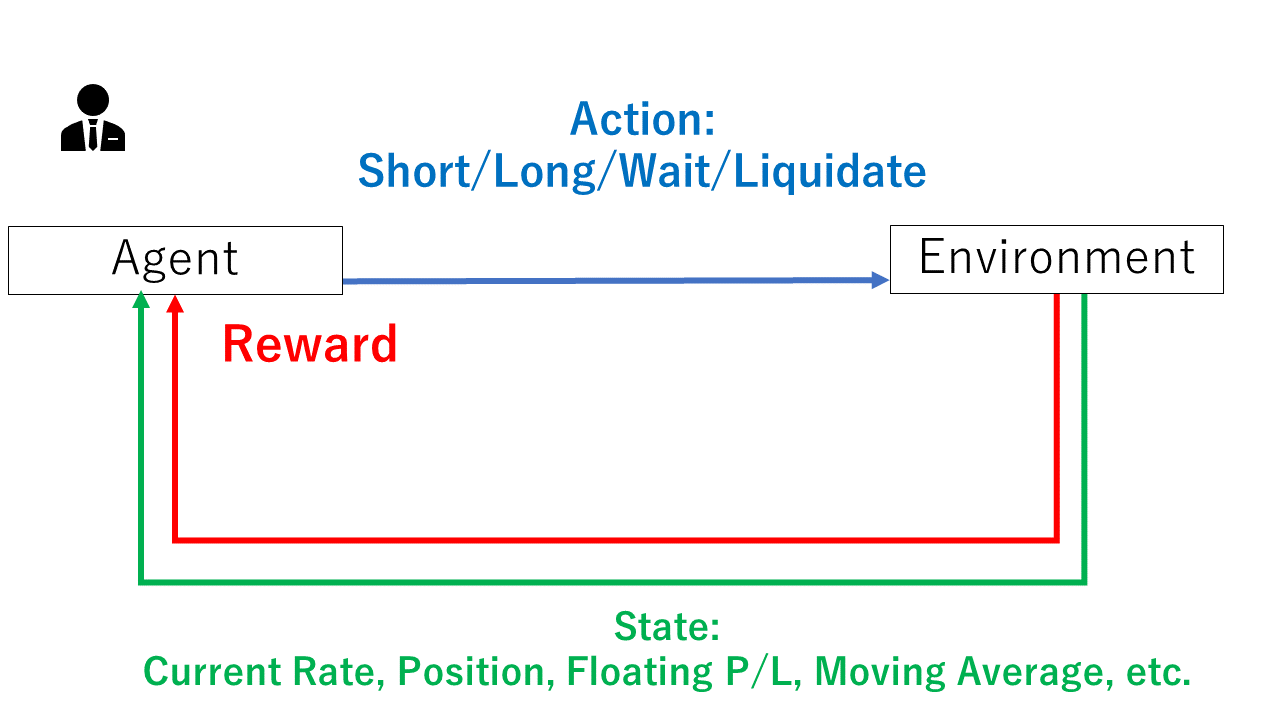
\includegraphics[scale=0.4]{./Figure/method_overview.png}
  \caption{RL for Forex trading}
  \label{fig:methodOverview}
\end{figure}

\section{State}
\label{sec:state}
The {\it state element} is defined as Equation (\ref{eq:state-el}) 
\begin{equation}
  \label{eq:state-el}
\mbox{ \boldmath{ $ S_{t} $}} = (cu_{t}, pos, ma1_{t}, ma2_{t}, ma3_{t}, ma4_{t}, ma5_{t}, fpl_{t}, pos\_rate).
\end{equation}
The subscript $t$ means {\it time step}, and the same applies hereafter. The $t$ starts with 120 to calculate the moving average $ma1_{t}$.

The $cu_{t}$ means {\it current exchange rate}.

Denoted as $pos$, the (\ref{eq:pos}) defines {\it current position} as
\begin{equation}
  \label{eq:pos}
   pos \in \{ SQUARE, SHORT, LONG \},
\end{equation}
where the agent is in.

Equation (\ref{eq:ma}) means {\it moving averages}:
\begin{equation}
  \label{eq:ma}
  \begin{array}{l}
    ma1_{t} = \frac{1}{120} \displaystyle \sum_{i=t-120}^{t} p_i, \\
    ma2_{t} = \frac{1}{80} \displaystyle \sum_{i=t-80}^{t} p_i,   \\
    ma3_{t} = \frac{1}{50} \displaystyle \sum_{i=t-50}^{t} p_i,   \\
    ma4_{t} = \frac{1}{30} \displaystyle \sum_{i=t-30}^{t} p_i,   \\
    ma5_{t} = \frac{1}{20} \displaystyle \sum_{i=t-20}^{t} p_i.   \\
  \end{array}
\end{equation}
The $p_i$ means the exchange rate (price) at the time step $i$.

Equation (\ref{eq:fpl-def}) means {\it floating P/L} which corresponds to Section \ref{sec:Forex}:
\begin{equation}
  \label{eq:fpl-def}
  fpl_{t} =
  \left\{
    \begin{array}{l}
      cu_{t} - pos\_rate  \ (pos=LONG)\\
      pos\_rate - cu_{t}  \ (pos=SHORT)\\
      0 \ (otherwise)
    \end{array}
  \right..
\end{equation}

The $pos\_rate$ means the {\it exchange rate when taking the position}. For example, the $pos\_rate=112.55$ means that the 1 dollar had equaled 112.55 yen when the agent had taken the long or the short position. If the agent is in the square, the $pos\_rate$ becomes zero.

\section{Deviation of Exchange Rate Data}
\label{sec:devEx}
In fact, all data of the exchange rate is normalized as Equation \ref{eq:normlize} 
\begin{equation}
  \label{eq:normlize}
  p_{t} = d_{t} - \frac{1}{N} \sum_{i=1}^{N} d_i,
\end{equation}
where the $N$ means the time period of the entire data history. The $d_t$ means original data of the dataset in Section \ref{sec:dataset}. The time period $N$ depends on the number of the data in Table \ref{tb:dataset}.

The normalization narrows the range between maximum and minimum in the state space to reduce computational complexity.

\section{Action}
\label{sec:action}
The {\it action set} $\mathcal{A}$ is defined as Equation (\ref{eq:action-set}):
\begin{equation}
  \label{eq:action-set}
  \begin{array}{l}
   \mathcal{A}( \mbox{\boldmath{$ pos=SQUARE $}} )=\{ WAIT, SHORT, LONG \} \\
   \mathcal{A}( \mbox{\boldmath{$ pos=ohterwise $}} )=\{ WAIT, LIQUIDATE \}.
  \end{array}
\end{equation}
Equation (\ref{eq:action-set}) corresponds to the position transition as Figure \ref{fig:pos_trans}.

The (\ref{eq:action-element}) shows each {\it action element} $A_{t}$ belongs to the action set. Each action element $A_{t}$ means taken action at time $t$.
\begin{equation}
  \label{eq:action-element}
  A_{t} \in \mathcal{A}( \mbox{\boldmath{$ pos $}} )
\end{equation}

\section{Action Modification}
\label{sec:actMod}
Despite Equation \ref{eq:action-set}, the agent may take wrong action. For example, he may liquidate wrongly even when he is in the square. This is because the agent must learn the position transition of Figure \ref{fig:pos_trans} although the transition is deterministic.

Therefore, the RL system is implemented to replace a wrong action with the {\it wait} action as below.
\begin{itemize}
  \item In Square: the agent wrongly {\it liquidates} $\Longrightarrow$  {\it wait} action
  \item In Short of Long position: the agent wrongly takes {\it long} or {\it short} position $\Longrightarrow$  {\it wait} action
\end{itemize}

In addition, the RL system forces the agent to liquidate his position forcefully when one episode finishes. If the system does not, the agent can keep waiting to avoid losses in any case even if he takes a long or short position.

\section{Episode}
The final time step $T$ of one episode is defined as Equation (\ref{eq:T-period}) 
\begin{equation}
  \label{eq:T-period}
  T = 1200.
\end{equation}

One {\it episode} is defined as the (\ref{eq:one-episode})  
\begin{equation}
  \label{eq:one-episode}
  \mbox{ \boldmath{ $ S_{0} $}}, A_{0}, \quad R_{1}, \mbox{ \boldmath{ $ S_{1} $}}, A_{1}, \quad R_{2}, \mbox{ \boldmath{ $ S_{2} $}}, A_{2}, \quad ...,\quad  R_{T-1}, \mbox{ \boldmath{ $ S_{T-1} $}}, A_{T-1}, \quad R_{T}, \mbox{ \boldmath{ $ S_{T} $}},
\end{equation}

One {\it step} is defined as Equation (\ref{eq:one-step})
\begin{equation}
  \label{eq:one-step}
  step = 
  \left\{
    \begin{array}{l}
      \mbox{ \boldmath{ $ S_{t} $}}, A_{t}       \qquad (t=0)\\
      R_{t}, \mbox{ \boldmath{ $ S_{t} $}}, A_{t} \ (otherwise)\\
    \end{array}
  \right.,
\end{equation}


\section{P/L and Reward}
\label{sec:pl_reward}
Equation (\ref{eq:pl-calc}) means profit and loss (P/L) which corresponds to Section \ref{sec:Forex}:
\begin{equation}
  \label{eq:pl-calc}
  profit =
  \left\{
    \begin{array}{l}
      (cu_{t} - pos\_rate) \times 10000  \ (pos=LONG \ \land \ a= LIQUIDATE)\\
      (pos\_rate - cu_{t}) \times 10000  \ (pos=SHORT\ \land \ a= LIQUIDATE)\\
      0                          \ (otherwise)\\
    \end{array}
  \right.,
\end{equation}
where $\times 10000$ is leverage to amplify P/L. The negative profit means losses.

Note that the $cu_{t}$ is the current exchange rate of time $t$, not $t+1$ of cover deal in Section \ref{sec:Forex}. It is simplification in order to make implementation easy.

In this research, the {\it reward} is defined as same as the profit. Note that the leverage enables the agent to learn because the normalization in Section \ref{sec:devEx} makes the reward without the leverage close to zero.

\section{DQN}
\label{sec:DQN}
As agent of RL, this research utilizes DQN \cite{mnih2013playing} where the policy is Boltzmann Q Policy, or soft-max policy.

The neural network is constructed with Keras as below:
\begin{lstlisting}[caption=Neural network structure with Keras, label=list:network]
  Layer (type)                 Output Shape              Param #   
  =================================================================
  flatten_1 (Flatten)          (None, 9)                 0         
  _________________________________________________________________
  dense_1 (Dense)              (None, 16)                160       
  _________________________________________________________________
  activation_1 (Activation)    (None, 16)                0         
  _________________________________________________________________
  dense_2 (Dense)              (None, 16)                272       
  _________________________________________________________________
  activation_2 (Activation)    (None, 16)                0         
  _________________________________________________________________
  dense_3 (Dense)              (None, 16)                272       
  _________________________________________________________________
  activation_3 (Activation)    (None, 16)                0         
  _________________________________________________________________
  dense_4 (Dense)              (None, 4)                 68        
  _________________________________________________________________
  activation_4 (Activation)    (None, 4)                 0         
  =================================================================
  Total params: 772
  Trainable params: 772
  Non-trainable params: 0
\end{lstlisting}

In Listing \ref{list:network}, the flatten\_1 layer is the input layer which takes the state elements as Equation \ref{eq:state-el}. The activation\_1, activation\_2, and activation\_3 layers utilize ReLU (Rectified Linear Unit) activation \cite{relu}, and the activation\_4 layer uses linear activation \cite{linear}. The dense\_1, dense\_2, dense\_3 and dense\_4 layers are densely-connected (fully-connected) neural network layers \cite{dense}. The activation\_4 corresponds to the output layer on the right side of Figure \ref{fig:QvsDQN} to decide to take an action as WAIT, SHORT, LONG or LIQUIDATE.

\chapter{Experiment}
\label{sec:experiment}
The agent is trained based on Section \ref{sec:method_algo} by 50,000 steps trading on the testing dataset which mostly equals 47 episodes. Each training episode consists of same data. After that, the agent is tested by trading of one episode on nine testing datasets. Note that each testing dataset make each environment interact with the agent exactly the same every episode. This is why testing consists of one episode.

To confirm the effect of MA as metrics, the training and nine testing vary the number of MA from zero to five. For example, when the number of MA is four which is denoted as MA4, the MA elements are changed as Equation \ref{eq:ma4}. When the number of MA is three which is denoted as MA3, the MA elements are changed as Equation \ref{eq:ma3}, and so on. 

\begin{equation}
  \label{eq:ma4}
  \begin{array}{l}
    ma1_{t} = \frac{1}{120} \displaystyle \sum_{i=t-120}^{t} p_i, \\
    ma2_{t} = \frac{1}{80} \displaystyle \sum_{i=t-80}^{t} p_i,   \\
    ma3_{t} = \frac{1}{50} \displaystyle \sum_{i=t-50}^{t} p_i,   \\
    ma4_{t} = \frac{1}{30} \displaystyle \sum_{i=t-30}^{t} p_i,   \\
    ma5_{t} = 0   \\
  \end{array}
\end{equation}

\begin{equation}
  \label{eq:ma3}
  \begin{array}{l}
    ma1_{t} = \frac{1}{120} \displaystyle \sum_{i=t-120}^{t} p_i, \\
    ma2_{t} = \frac{1}{80} \displaystyle \sum_{i=t-80}^{t} p_i,   \\
    ma3_{t} = \frac{1}{50} \displaystyle \sum_{i=t-50}^{t} p_i,   \\
    ma4_{t} = 0,   \\
    ma5_{t} = 0   \\
  \end{array}
\end{equation}

\section{Dataset}
\label{sec:dataset}
The dataset consists of the USD/JPY (US Dollar vs. Japanese Yen) exchange rate where the candlestick range is five minutes. It is comprised of the training dataset and nine testing datasets as Table \ref{tb:dataset} shows. Note that the trained/tested data are not the entire ones but 1200 ones that correspond to Equation \ref{eq:T-period}, which is listed as Trained/Tested Data Period column on Table \ref{tb:dataset}.

\begin{table}[htb]
  \centering
  \caption{Dataset of training and testing}
  \label{tb:dataset}
  \begin{tabular}{|c|c|c|c|}
  \hline
    Dataset Name & Period (Day.Month.Year, GMT)  & Number of Data & Trained/Tested Data Period \\
  \hline
    Train        & 01.01.2004 - 09.01.2004  & 1908           & 01.01.2004 - 07.01.2004  \\
    Test 1       & 11.01.2004 - 20.01.2004  & 2040           & 11.01.2004 - 16.01.2004  \\
    Test 2       & 01.02.2004 - 10.02.2004  & 2040           & 01.02.2004 - 06.02.2004  \\
    Test 3       & 20.06.2004 - 30.06.2004  & 2340           & 20.06.2004 - 25.06.2004  \\
    Test 4       & 02.01.2005 - 10.01.2005  & 1752           & 02.01.2005 - 07.01.2005  \\
    Test 5       & 01.01.2007 - 10.01.2007  & 2302           & 01.01.2007 - 05.01.2007  \\
    Test 6       & 01.01.2009 - 09.01.2009  & 1992           & 01.01.2009 - 07.01.2009  \\
    Test 7       & 02.01.2011 - 10.01.2011  & 1752           & 02.01.2011 - 07.01.2011  \\
    Test 8       & 01.01.2014 - 10.01.2014  & 2016           & 01.01.2014 - 08.01.2014  \\
    Test 9       & 01.01.2019 - 10.01.2019  & 2040           & 01.01.2019 - 08.01.2019  \\
  \hline
  \end{tabular}
\end{table}

\section{Evaluation Method}
\label{sec:evaluation}
The evaluation method consists of two parts: accumulated reward and waiting ratio. 

The first evaluation method is the {\it accumulated reward} which is defined as total rewards per one episode. It means the performance of agent's Forex trading. Note that the accumulated reward is equivalent to total P/L per one episode due to the definition of Section \ref{sec:pl_reward}.

The second evaluation method is the {\it waiting ratio} defined as Equation \ref{eq:waiting_def}
\begin{equation}
  \label{eq:waiting_def}
  \begin{array}{l}
    waiting \ ratio = \frac{the \ number \ of \ waiting \ in \ one \ episode}{the \ number \ of \ total \ actions \ in \ one \ episode}. \\
  \end{array}
\end{equation}
As mentioned in Section \ref{sec:motivation}, when a trader cannot be sure the direction of the exchange rate, he should wait. The waiting ratio shows whether RL realizes this strategy. The further the period of testing dataset is from the training period, the more the waiting ratio should increase.


\section{Details}
For details about source code and dataset, see the GitHub repository \cite{src}.

\chapter{Result}
\label{sec:result}
\section{Accumulated Reward}
Figure \ref{fig:acRewardTrain} shows the accumulated reward of each MA for each training episode. It suggests that the agent cannot learn how to make a profit because even the second half of the episodes show mostly negative rewards, as well as Table \ref{tb:acRewardTrain10} shows. In addition, the number of MA seems to have little impact on the reward in the training.


\begin{figure}[htbp]
  \centering
  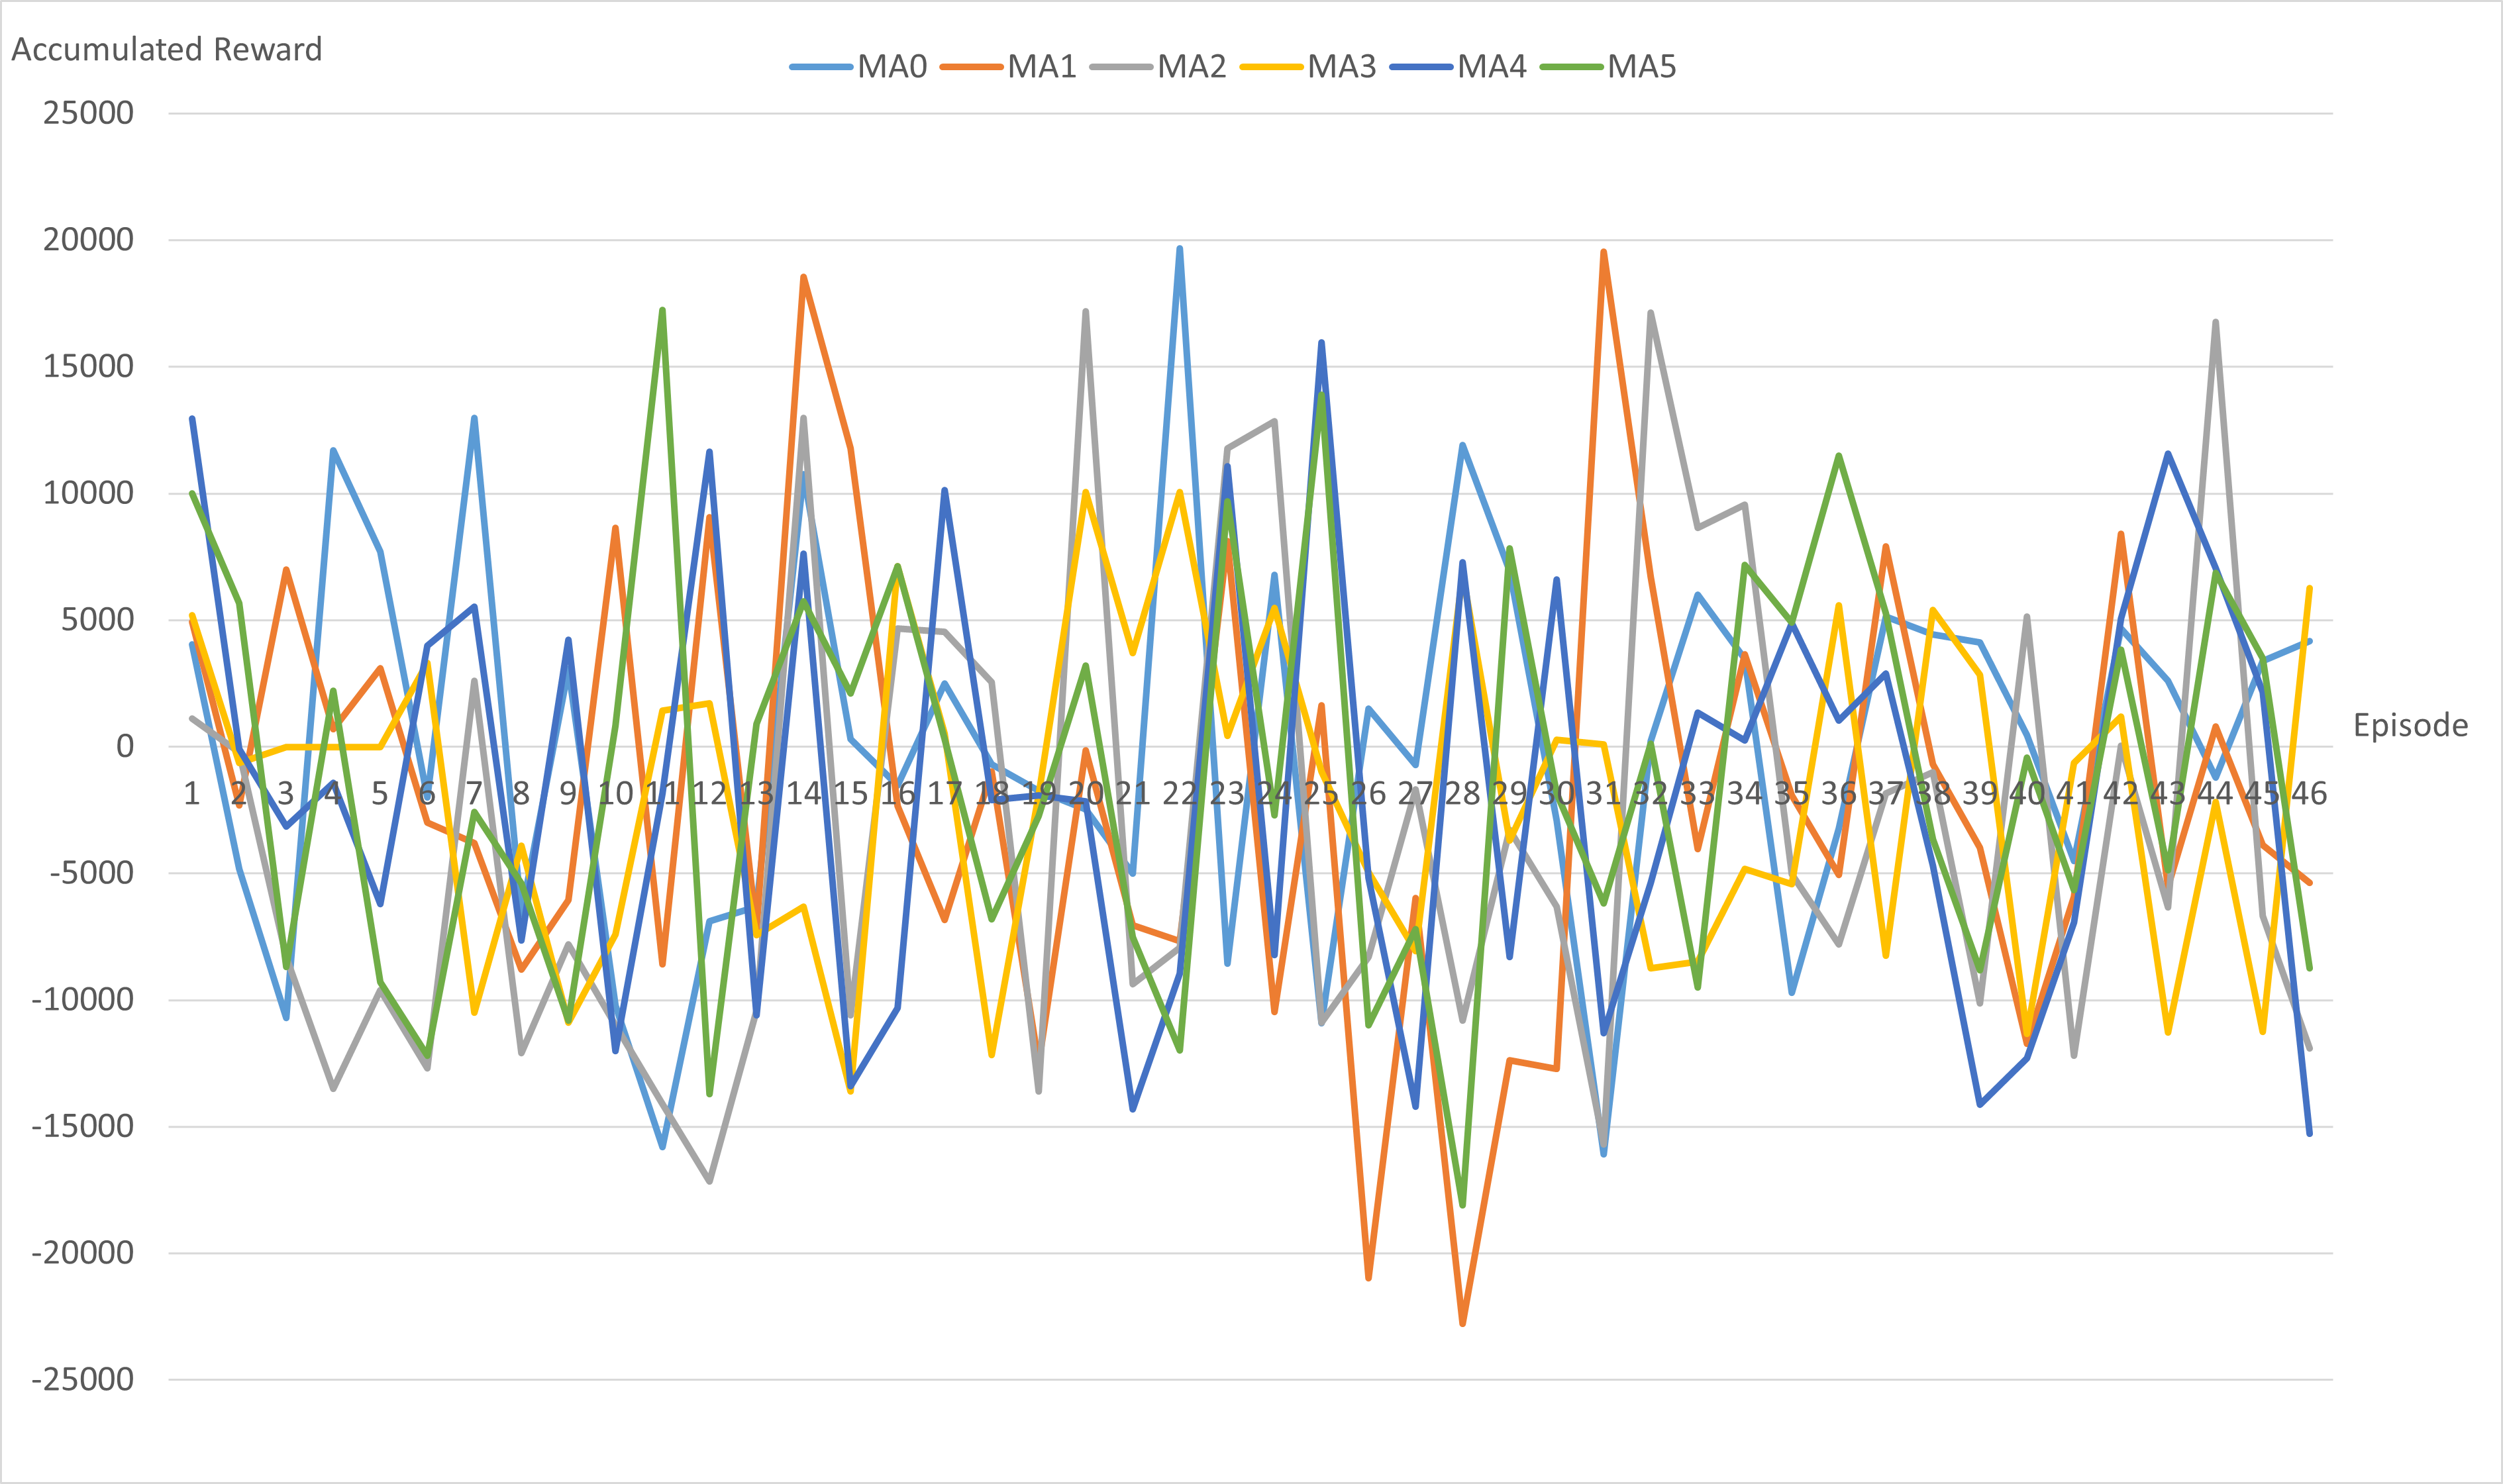
\includegraphics[scale=0.5]{./Figure/acRewardTrain.png}
  \caption{Accumulated reward in training for the number of moving average (MA)}
  \label{fig:acRewardTrain}
\end{figure}

\begin{table}[htb]
  % Source: The row "last 10 avg." of rewardVStrain_formatted.xlsx
  \centering
  \caption{The average of accumulated reward in the last ten trainings for each MA}
  \label{tb:acRewardTrain10}
  \begin{tabular}{|c|c|c|c|c|c|}
  \hline
    MA0  & MA1   & MA2    & MA3   & MA4    & MA5   \\
  \hline
    954  & -2748 & -2169  & -2785 & -2123  & -1205 \\
  \hline
  \end{tabular}
\end{table}

The same is true for Figure \ref{fig:acRewardTest}. Most rewards of the tests are negative, and the figure suggests that the number of MA could not improve the trading performance since each MA shows similar accumulated rewards. If the number of MA had some sort of impact on the performance, each MA would show the different accumulated reward.

As a result, it is concluded that MA may be invalid metrics for DQL of Forex trading.
\begin{figure}[htbp]
  \centering
  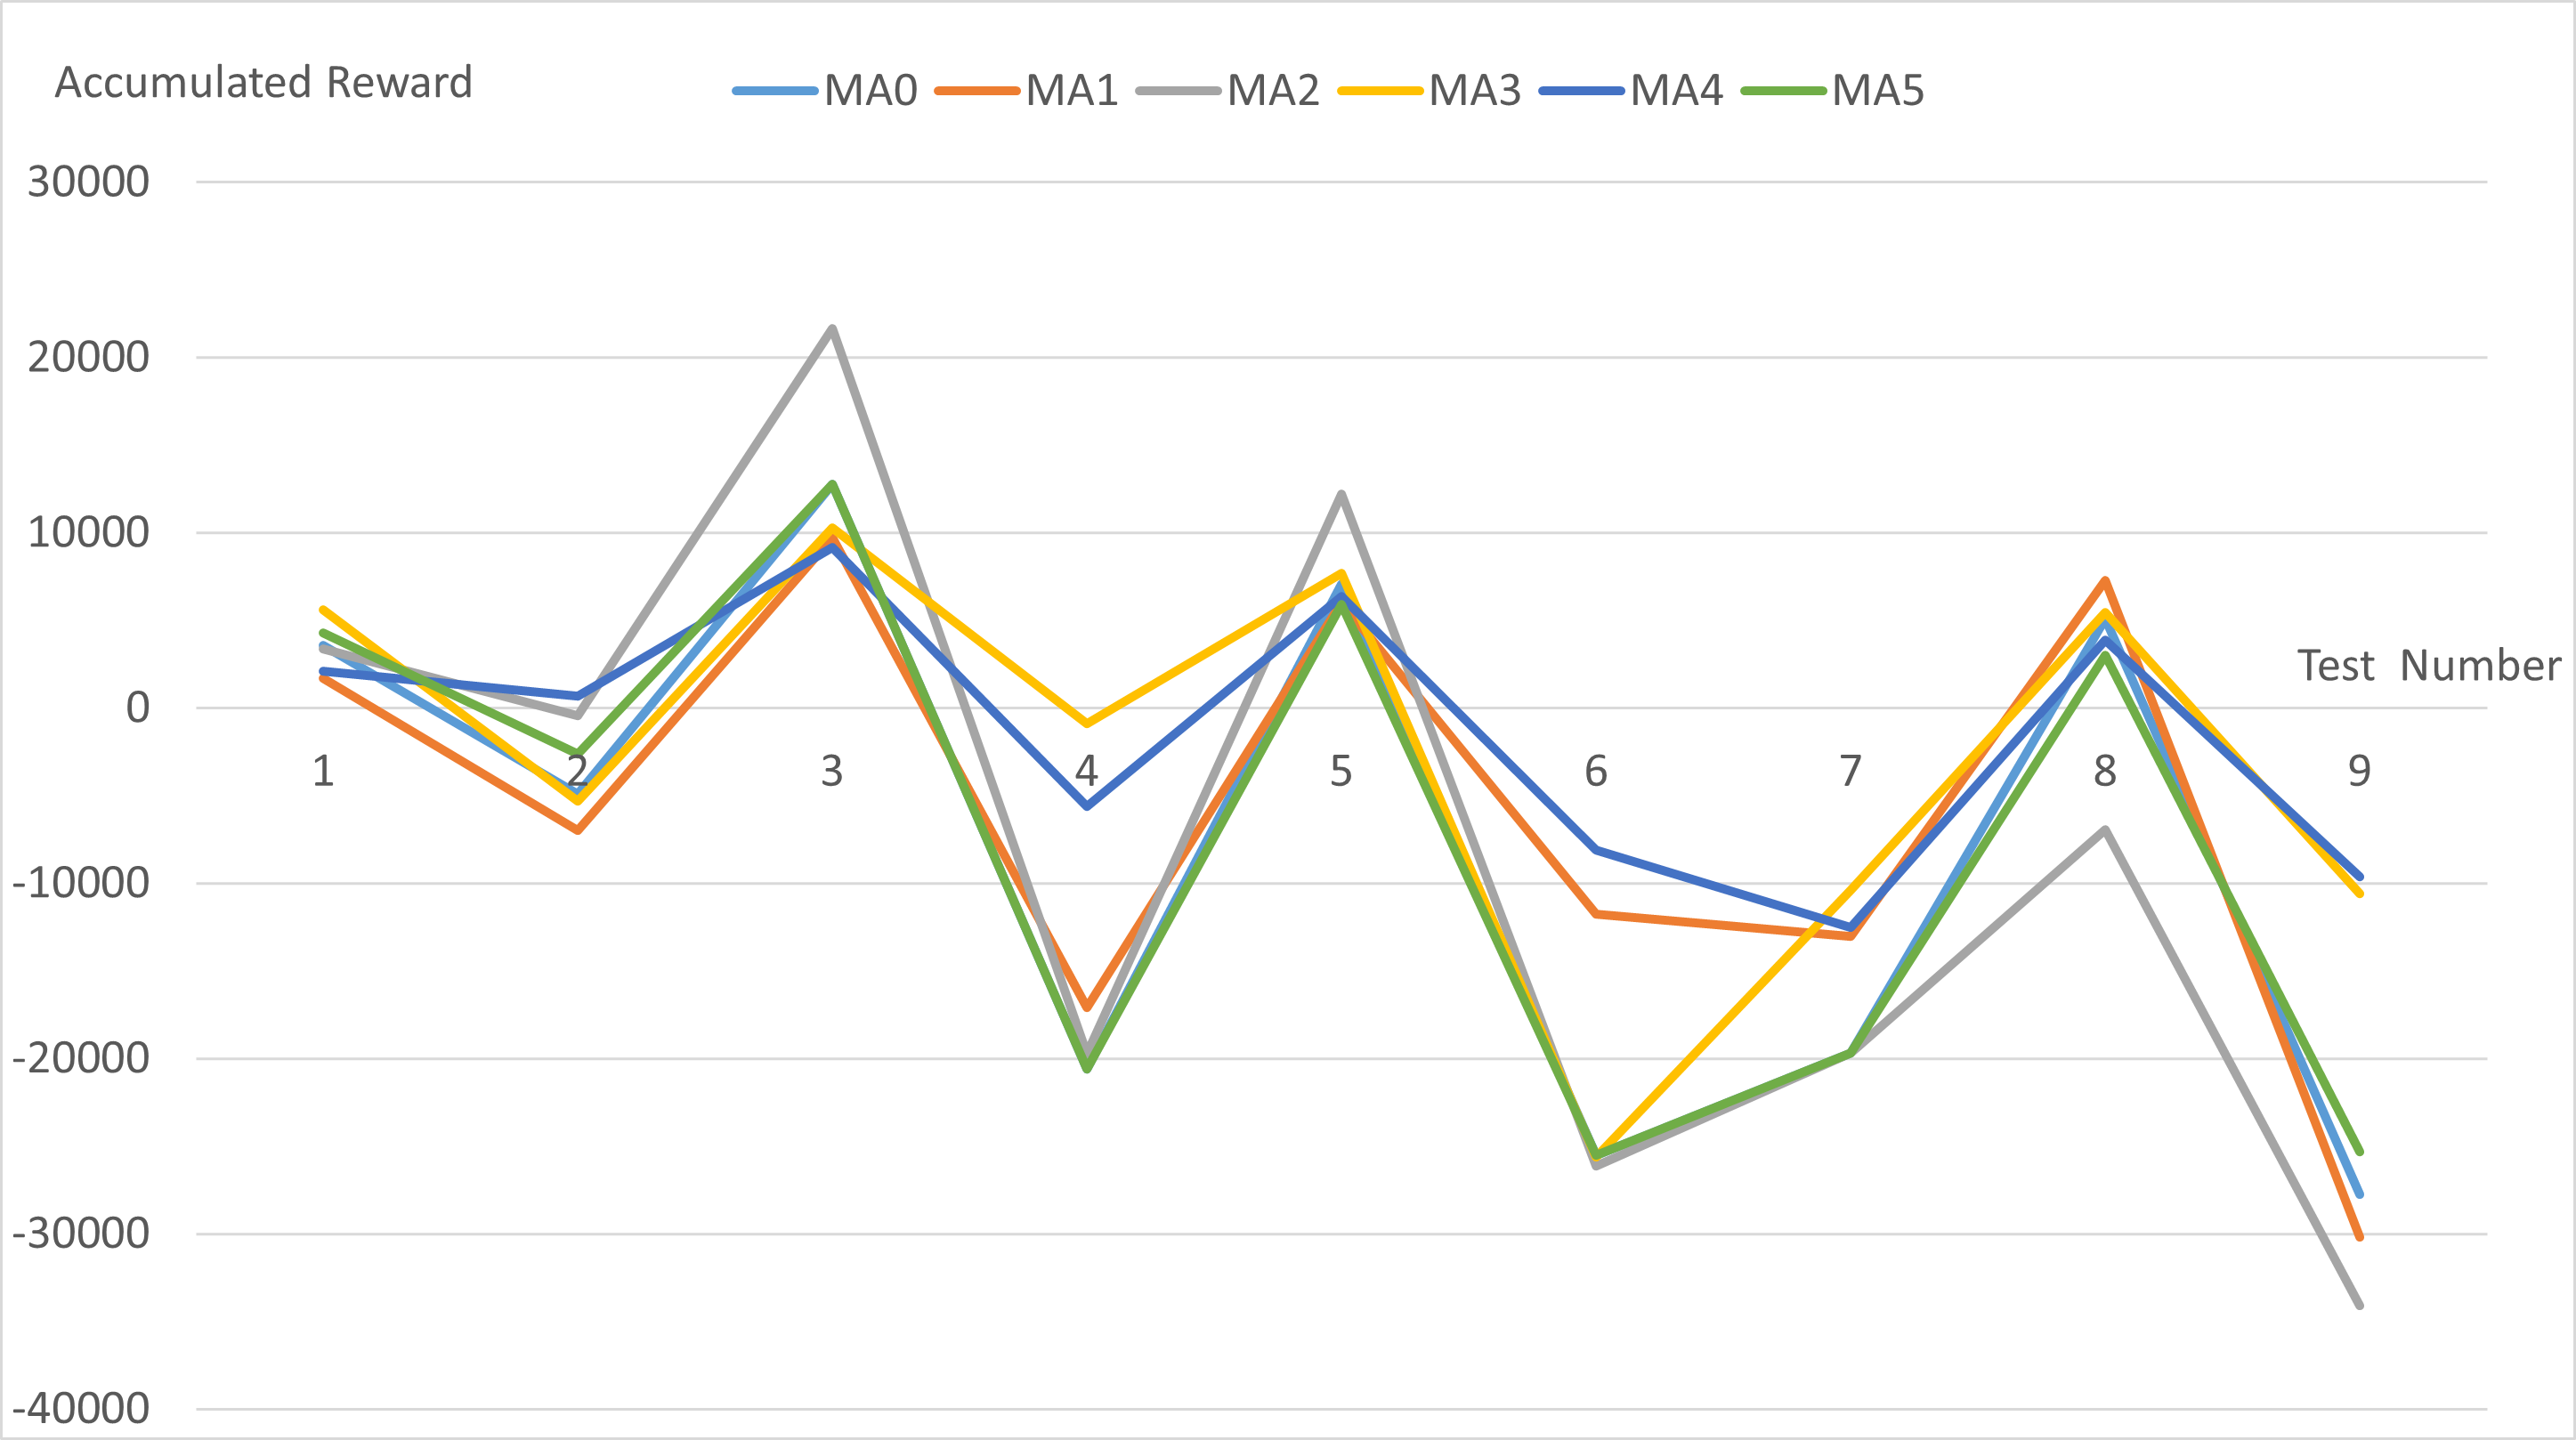
\includegraphics[scale=0.5]{./Figure/acRewardTest.png}
  \caption{Accumulated reward in testing for the number of MA}
  \label{fig:acRewardTest}
\end{figure}


\section{Waiting Ratio}
\label{sec:waitingRatioResult}
Figure \ref{fig:waitingTrain} is the chart of the waiting ratio for each MA in the training episodes. It suggests that the waiting ratios of any number of MA tend to converge to the range of 70\% to 75\% as well as Figure \ref{fig:waitingTrainAvg} shows. 

From Figure \ref{fig:ma0waitingReward} to Figure \ref{fig:ma5waitingReward}, these figures indicate that the range of 70\% to 75\% is the boundary whether the loss absolutely occurs or not: the right sides of the range in the figures show that most data points are negative accumulated rewards.

RL is presumed to help to avoid losses in Forex trading. As explained in the previous section, it was difficult for the agent to get profit with MA metrics, therefore the agent seemingly focuses on avoiding losses. 

\begin{figure}[htbp]
  \centering
  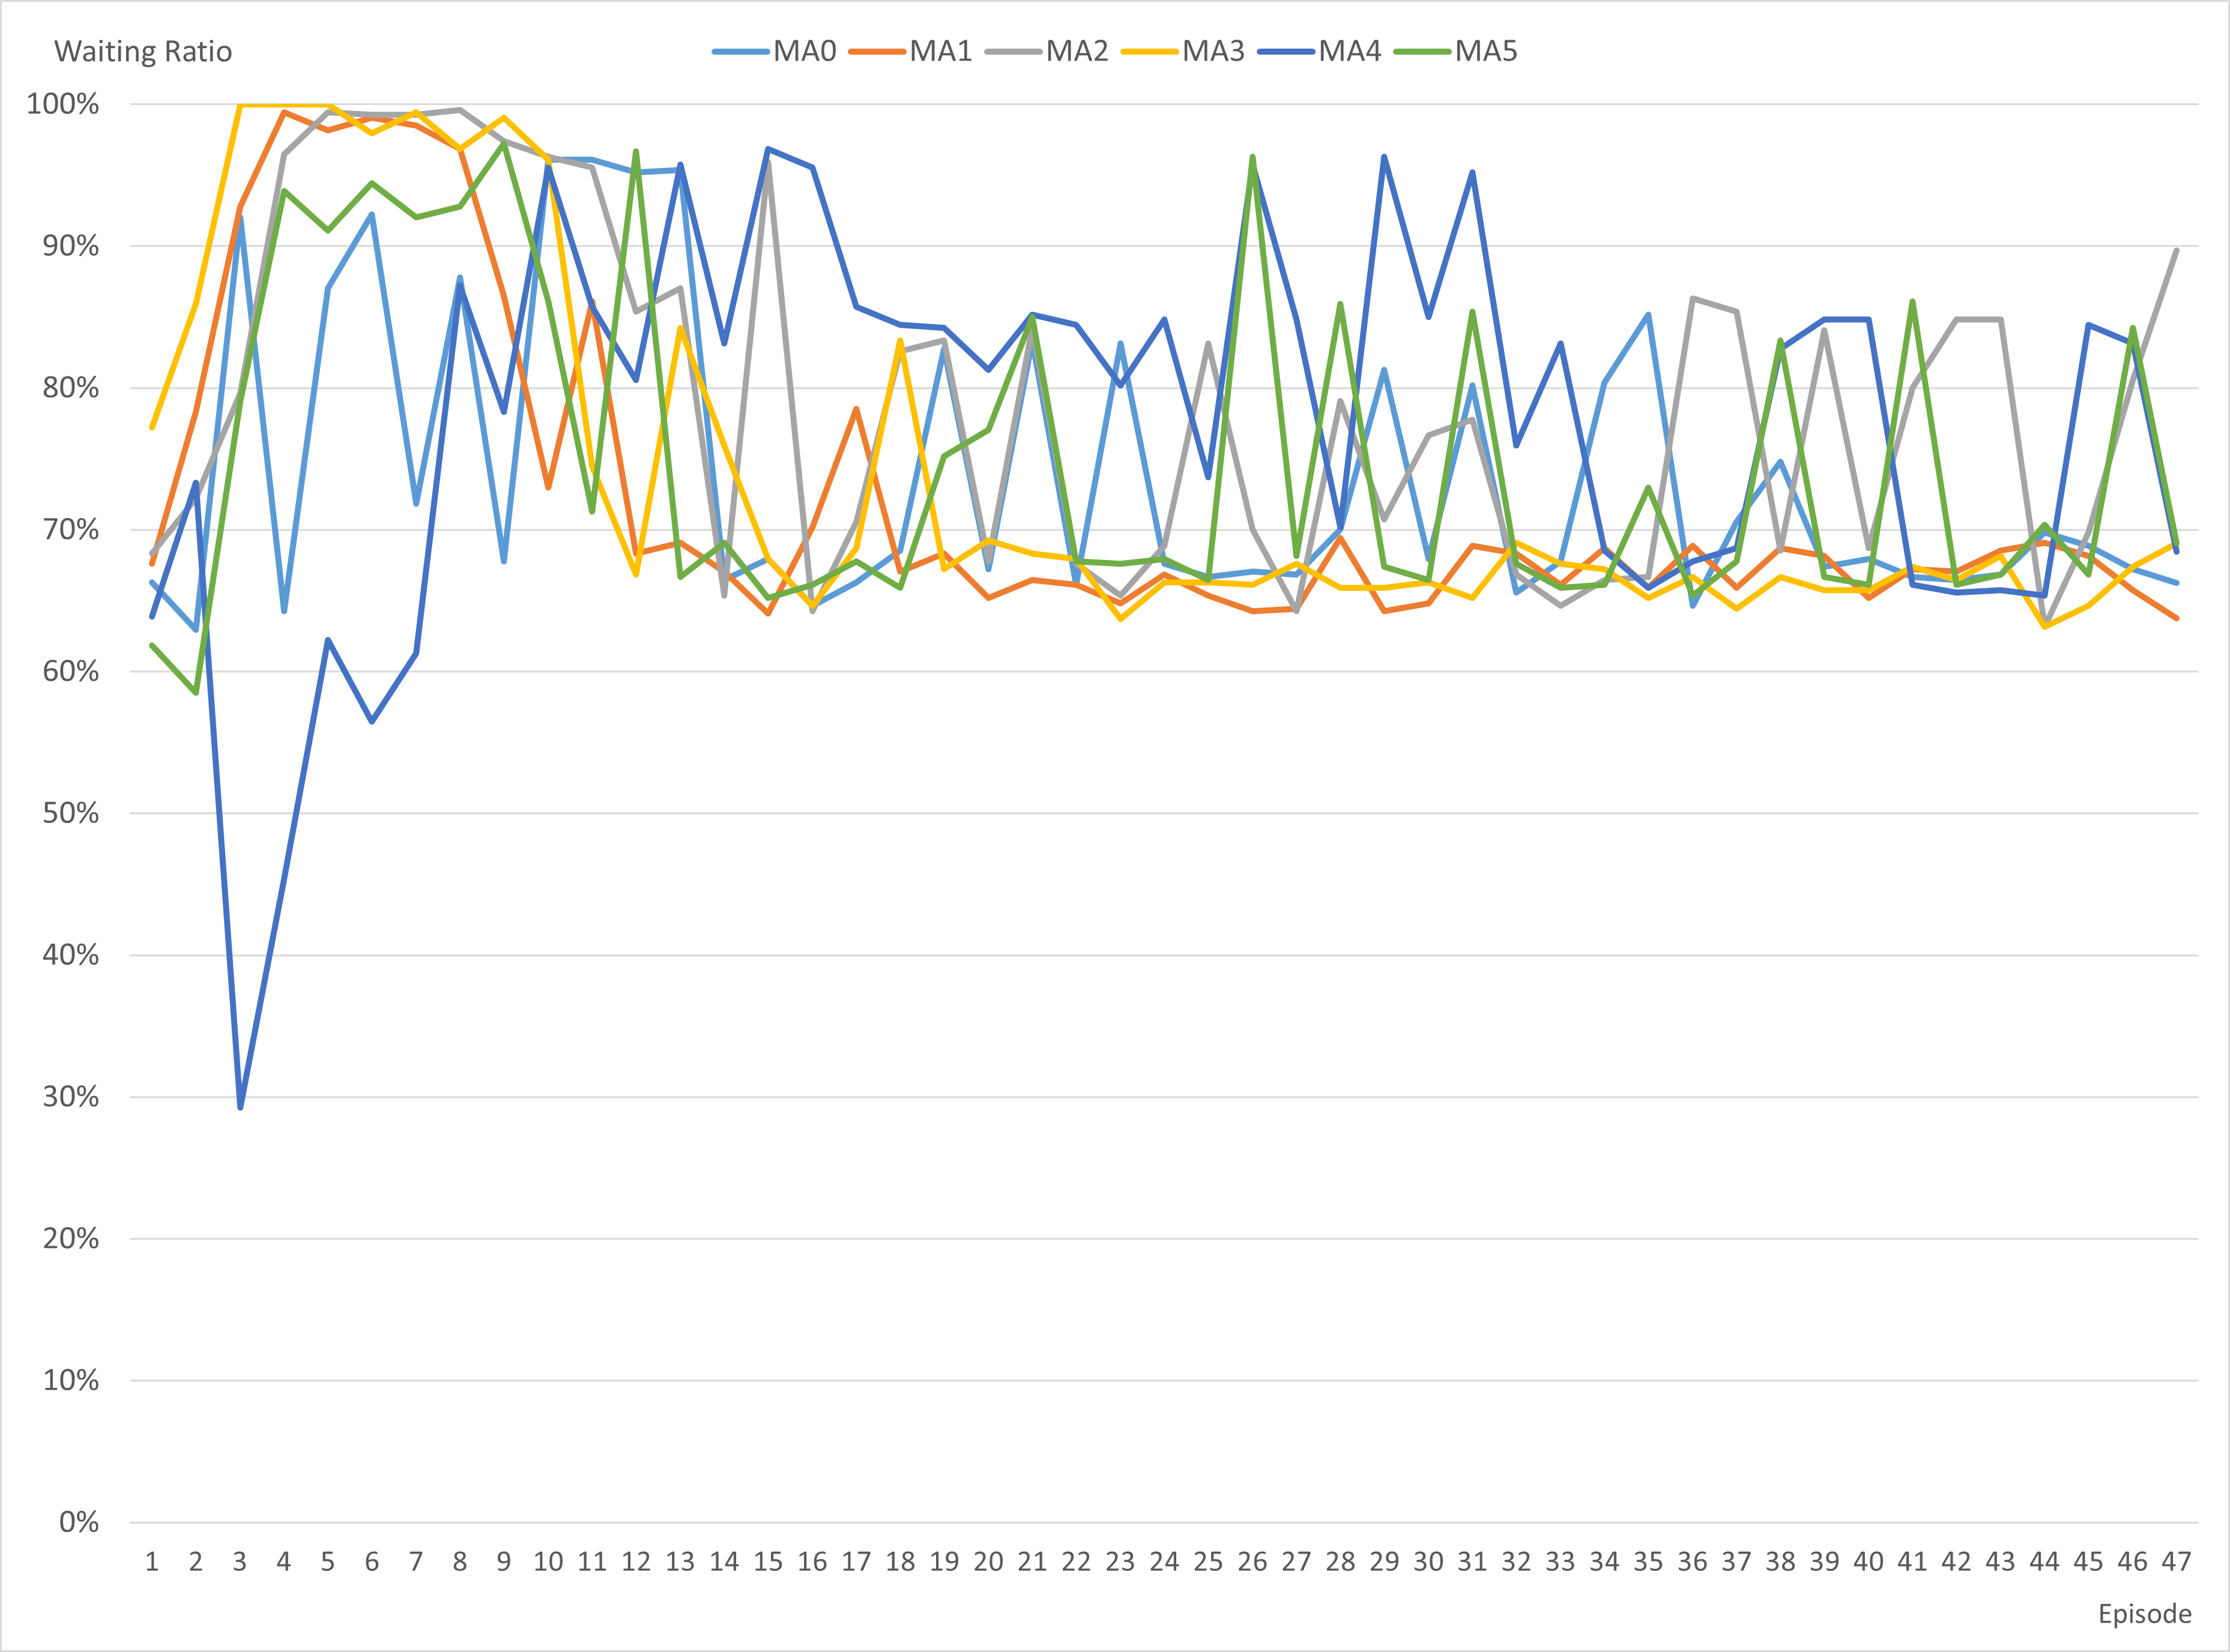
\includegraphics[scale=0.5]{./Figure/waitingTrain.png}
  \caption{Waiting ratio in training for the number of MA}
  \label{fig:waitingTrain}
\end{figure}

\begin{figure}[htbp]
  \centering
  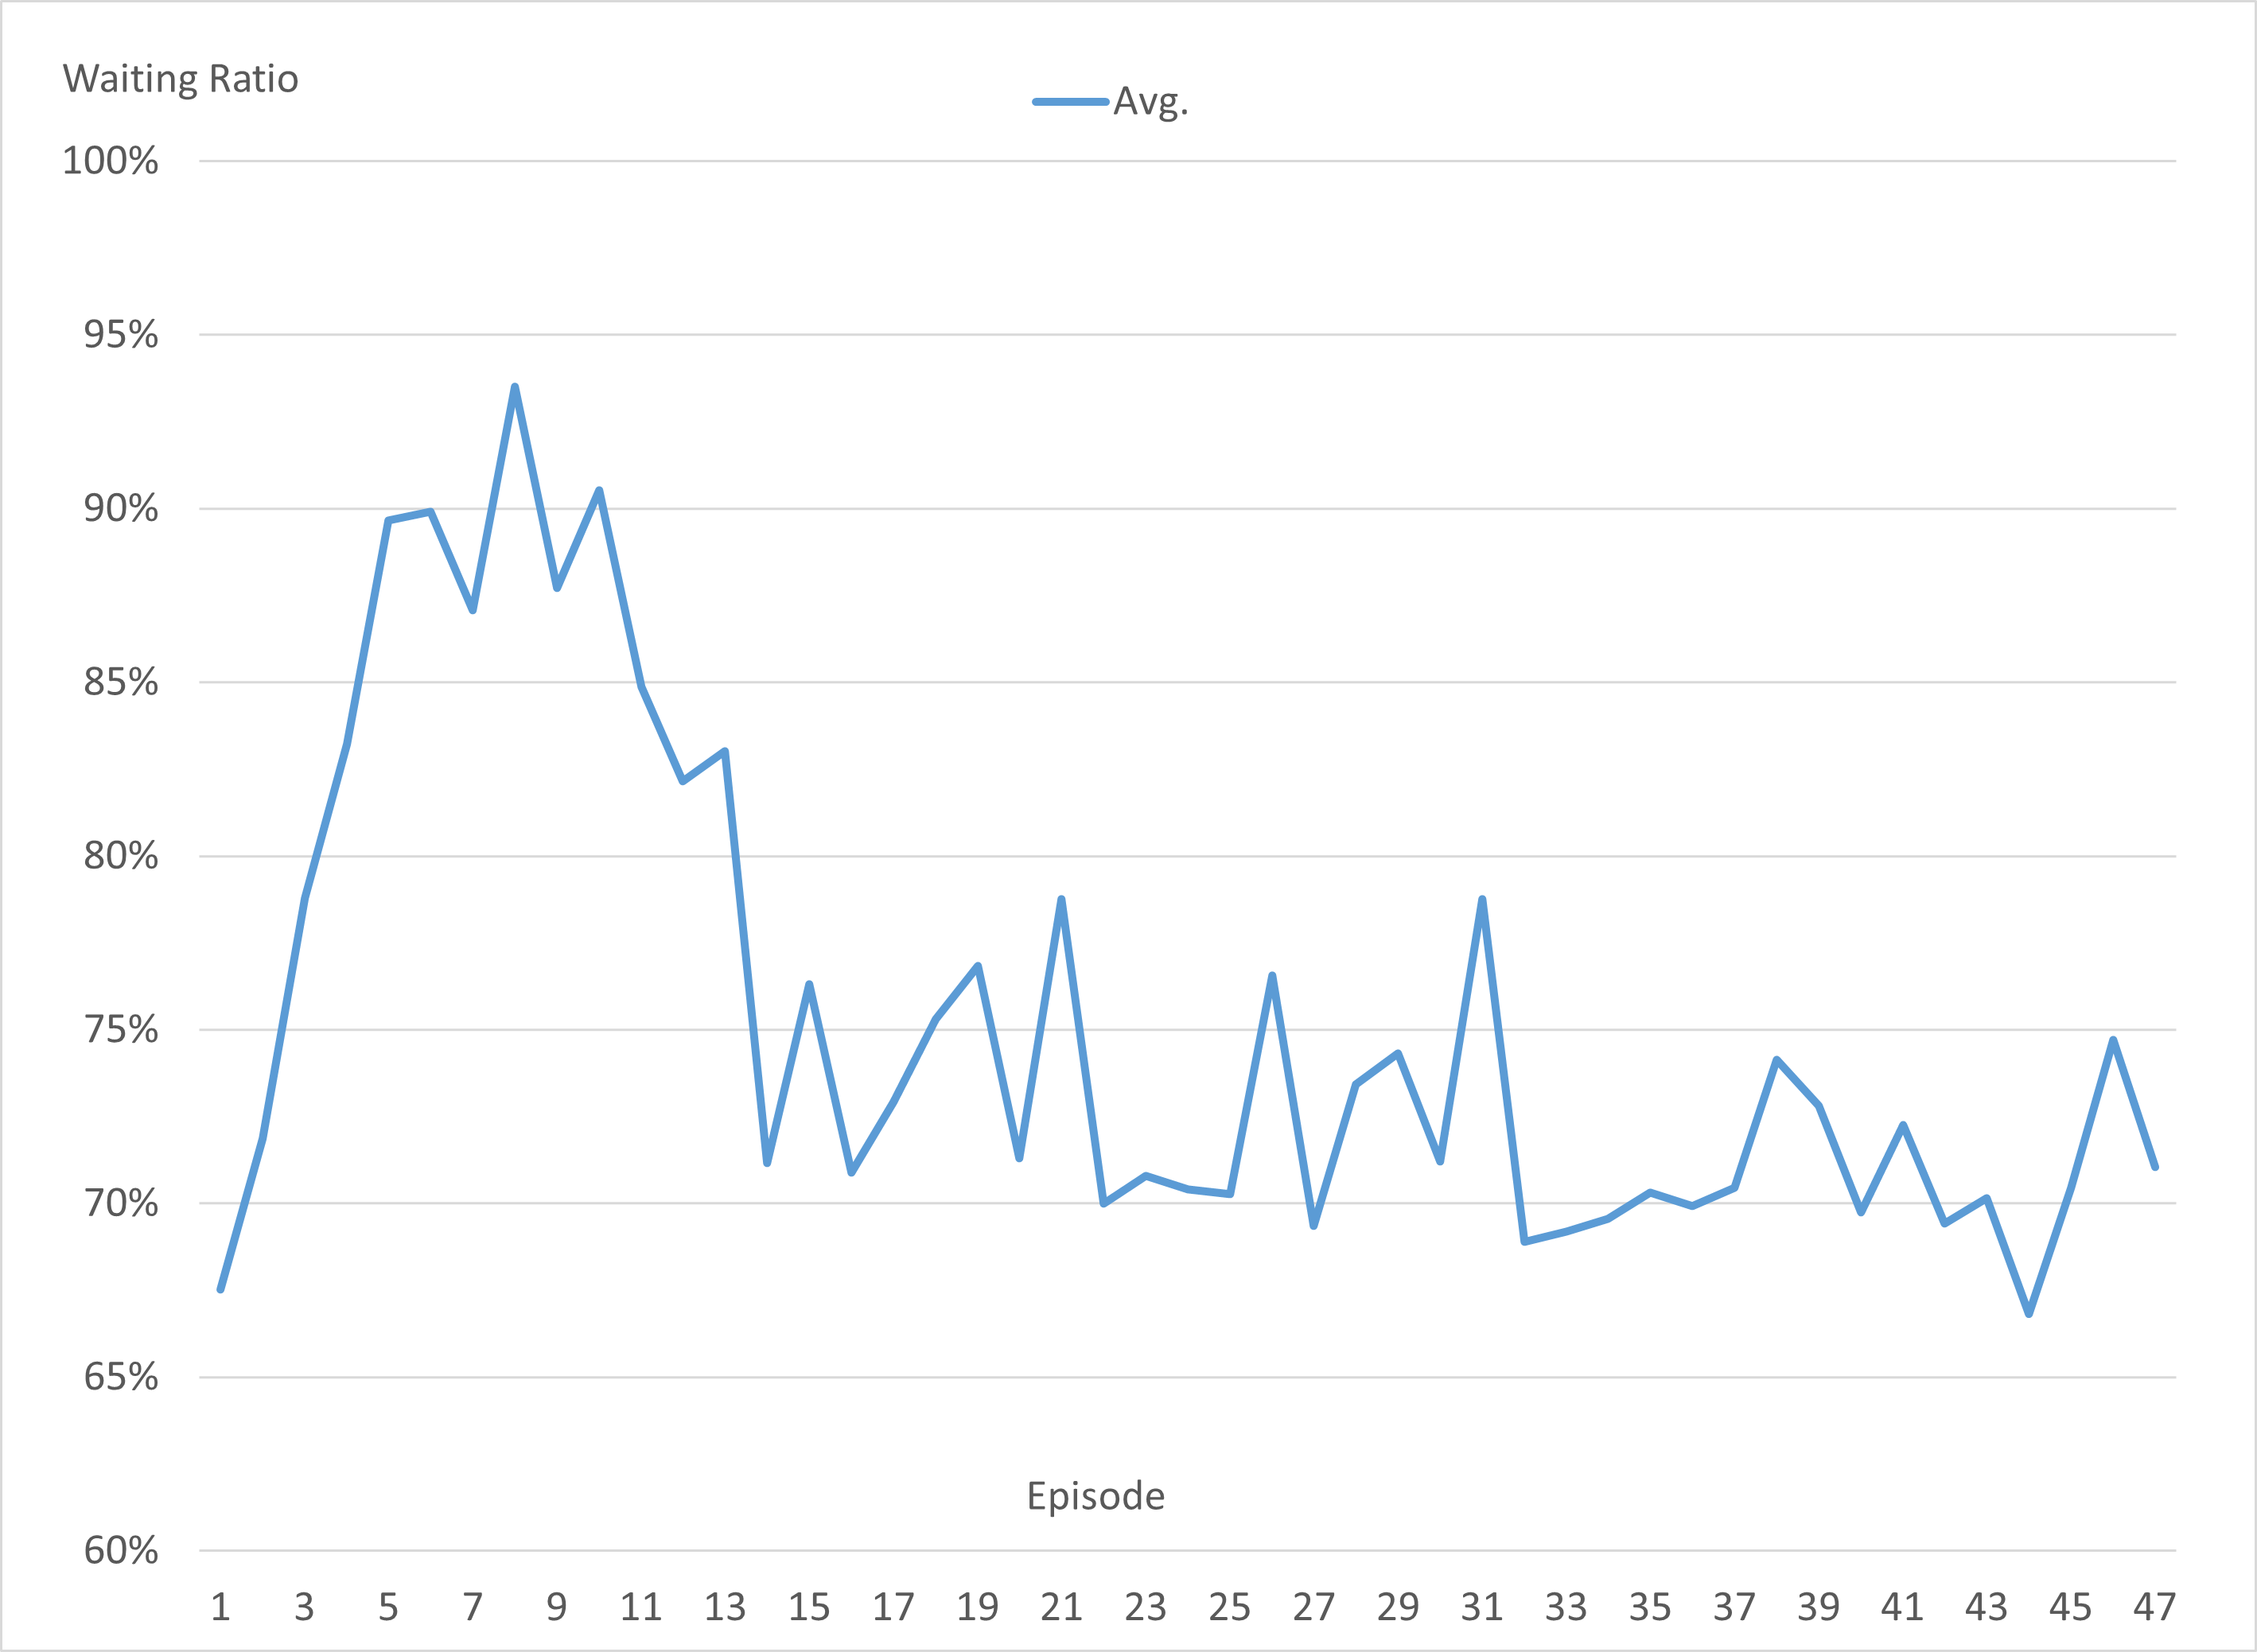
\includegraphics[scale=0.5]{./Figure/waitingTrainAvg.png}
  \caption{Average of waiting ratio in testing for the number of MA}
  \label{fig:waitingTrainAvg}
\end{figure}

\begin{figure}[htbp]
  \centering
  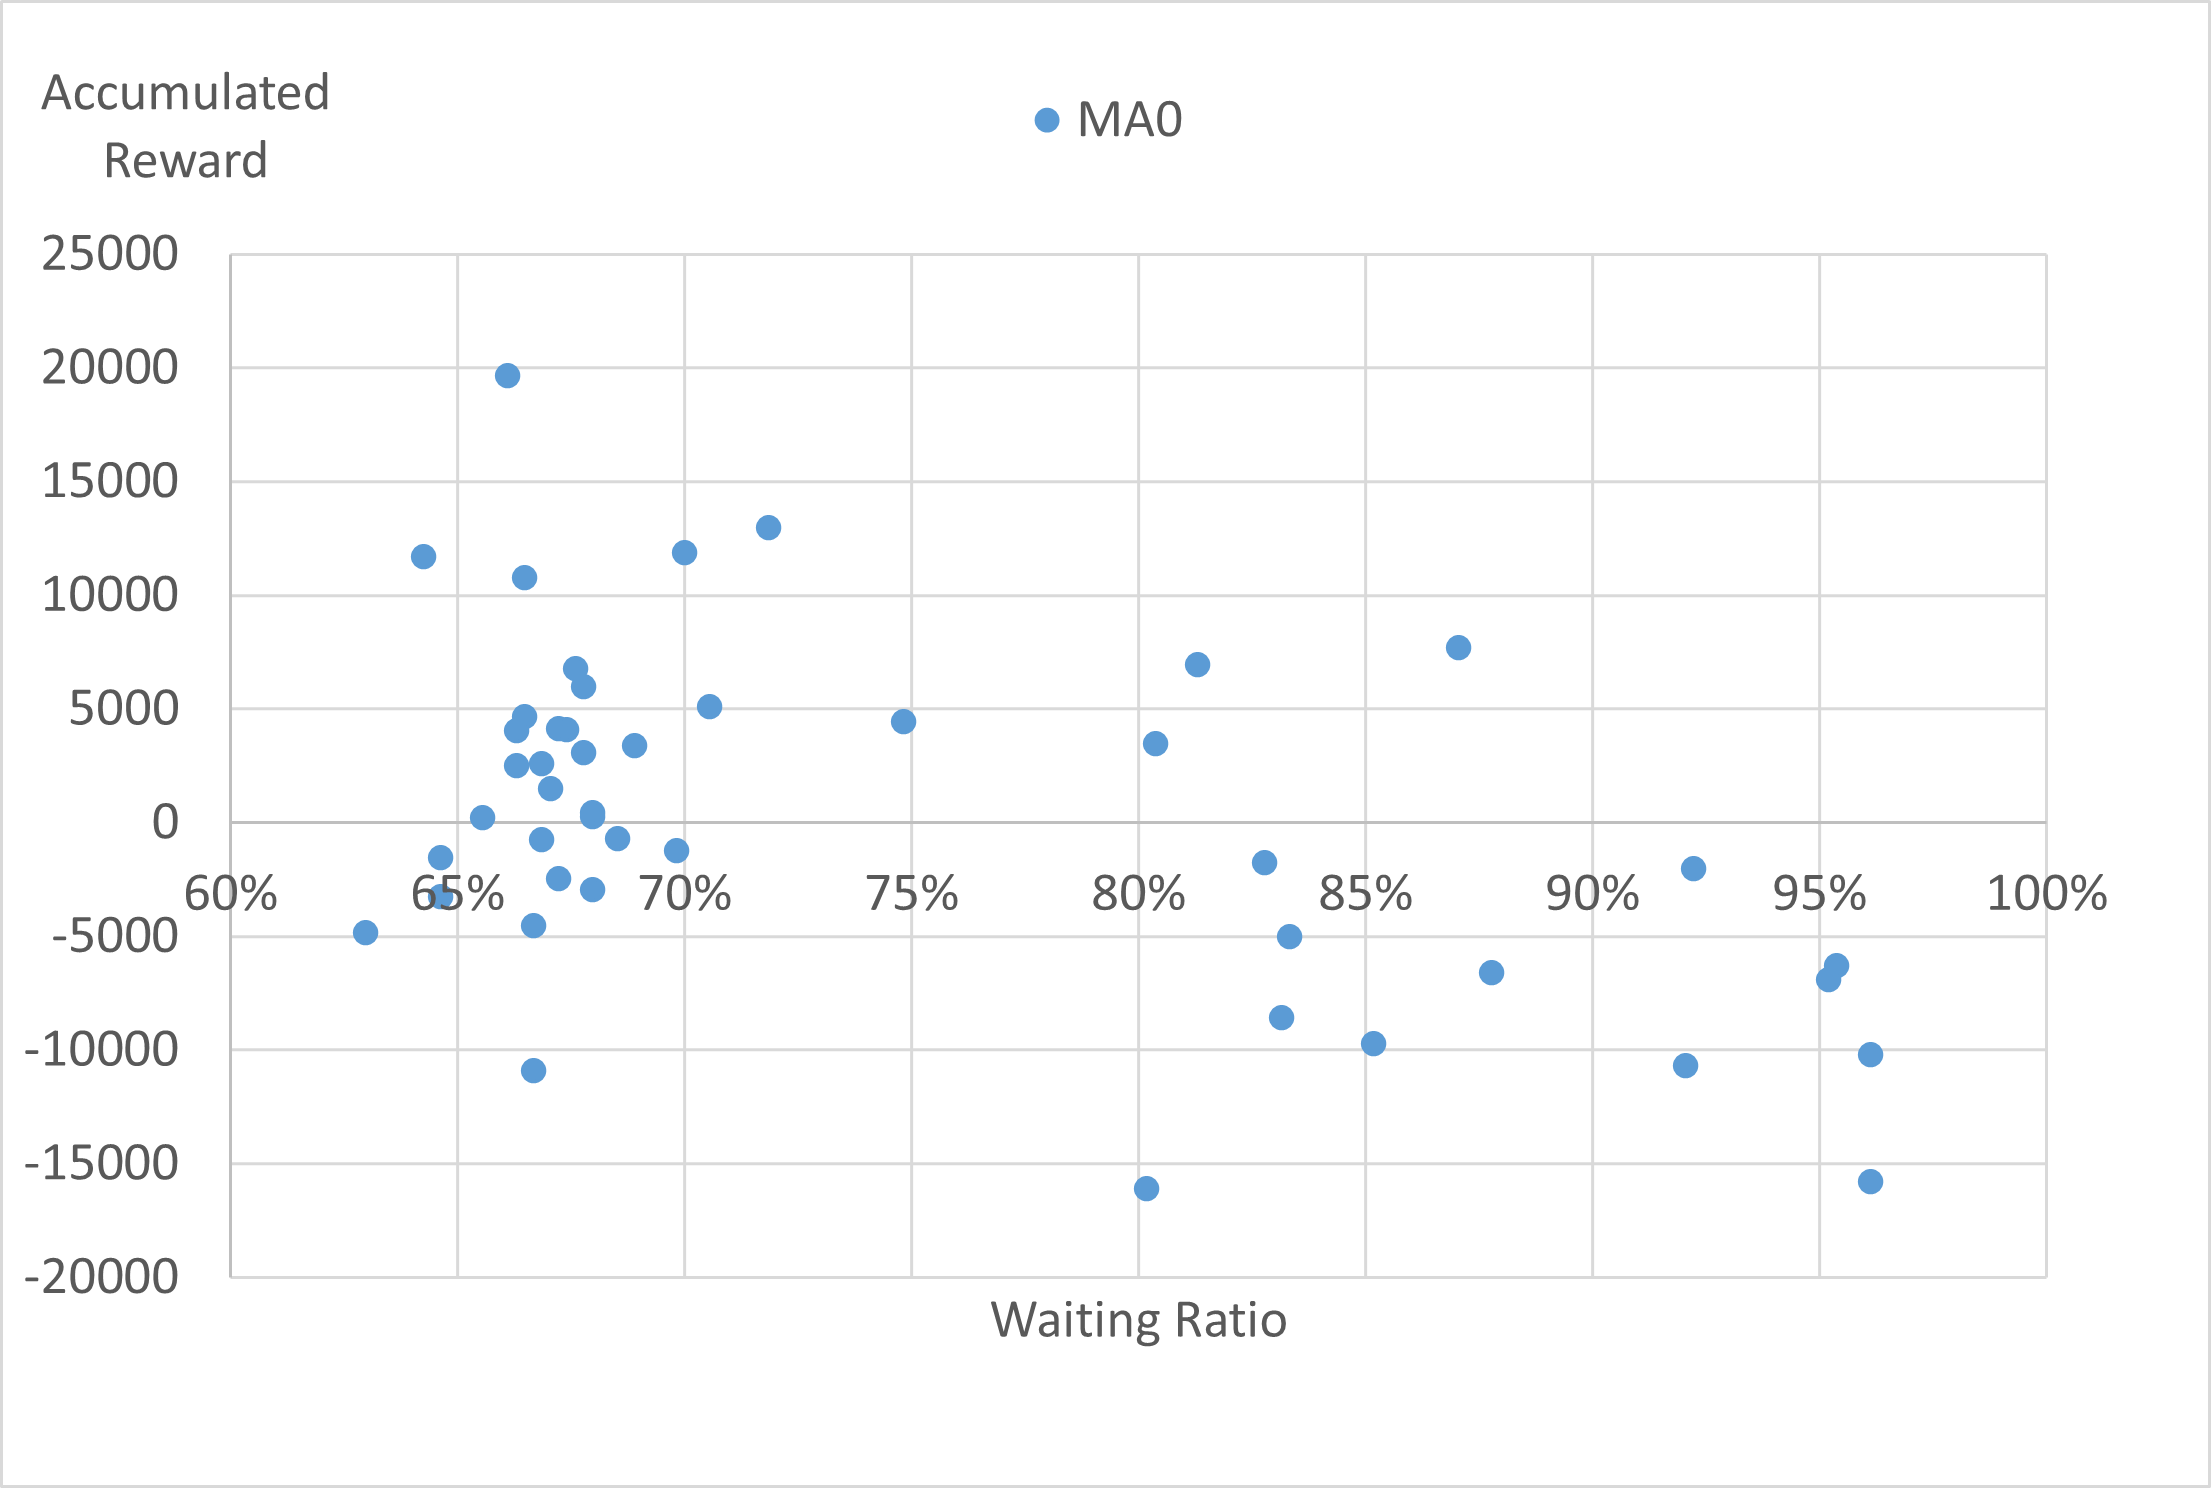
\includegraphics[scale=0.5]{./Figure/ma0waitingReward.png}
  \caption{Scatter plot between waiting ratio and accumulated reward in training of MA0}
  \label{fig:ma0waitingReward}
\end{figure}

\begin{figure}[htbp]
  \centering
  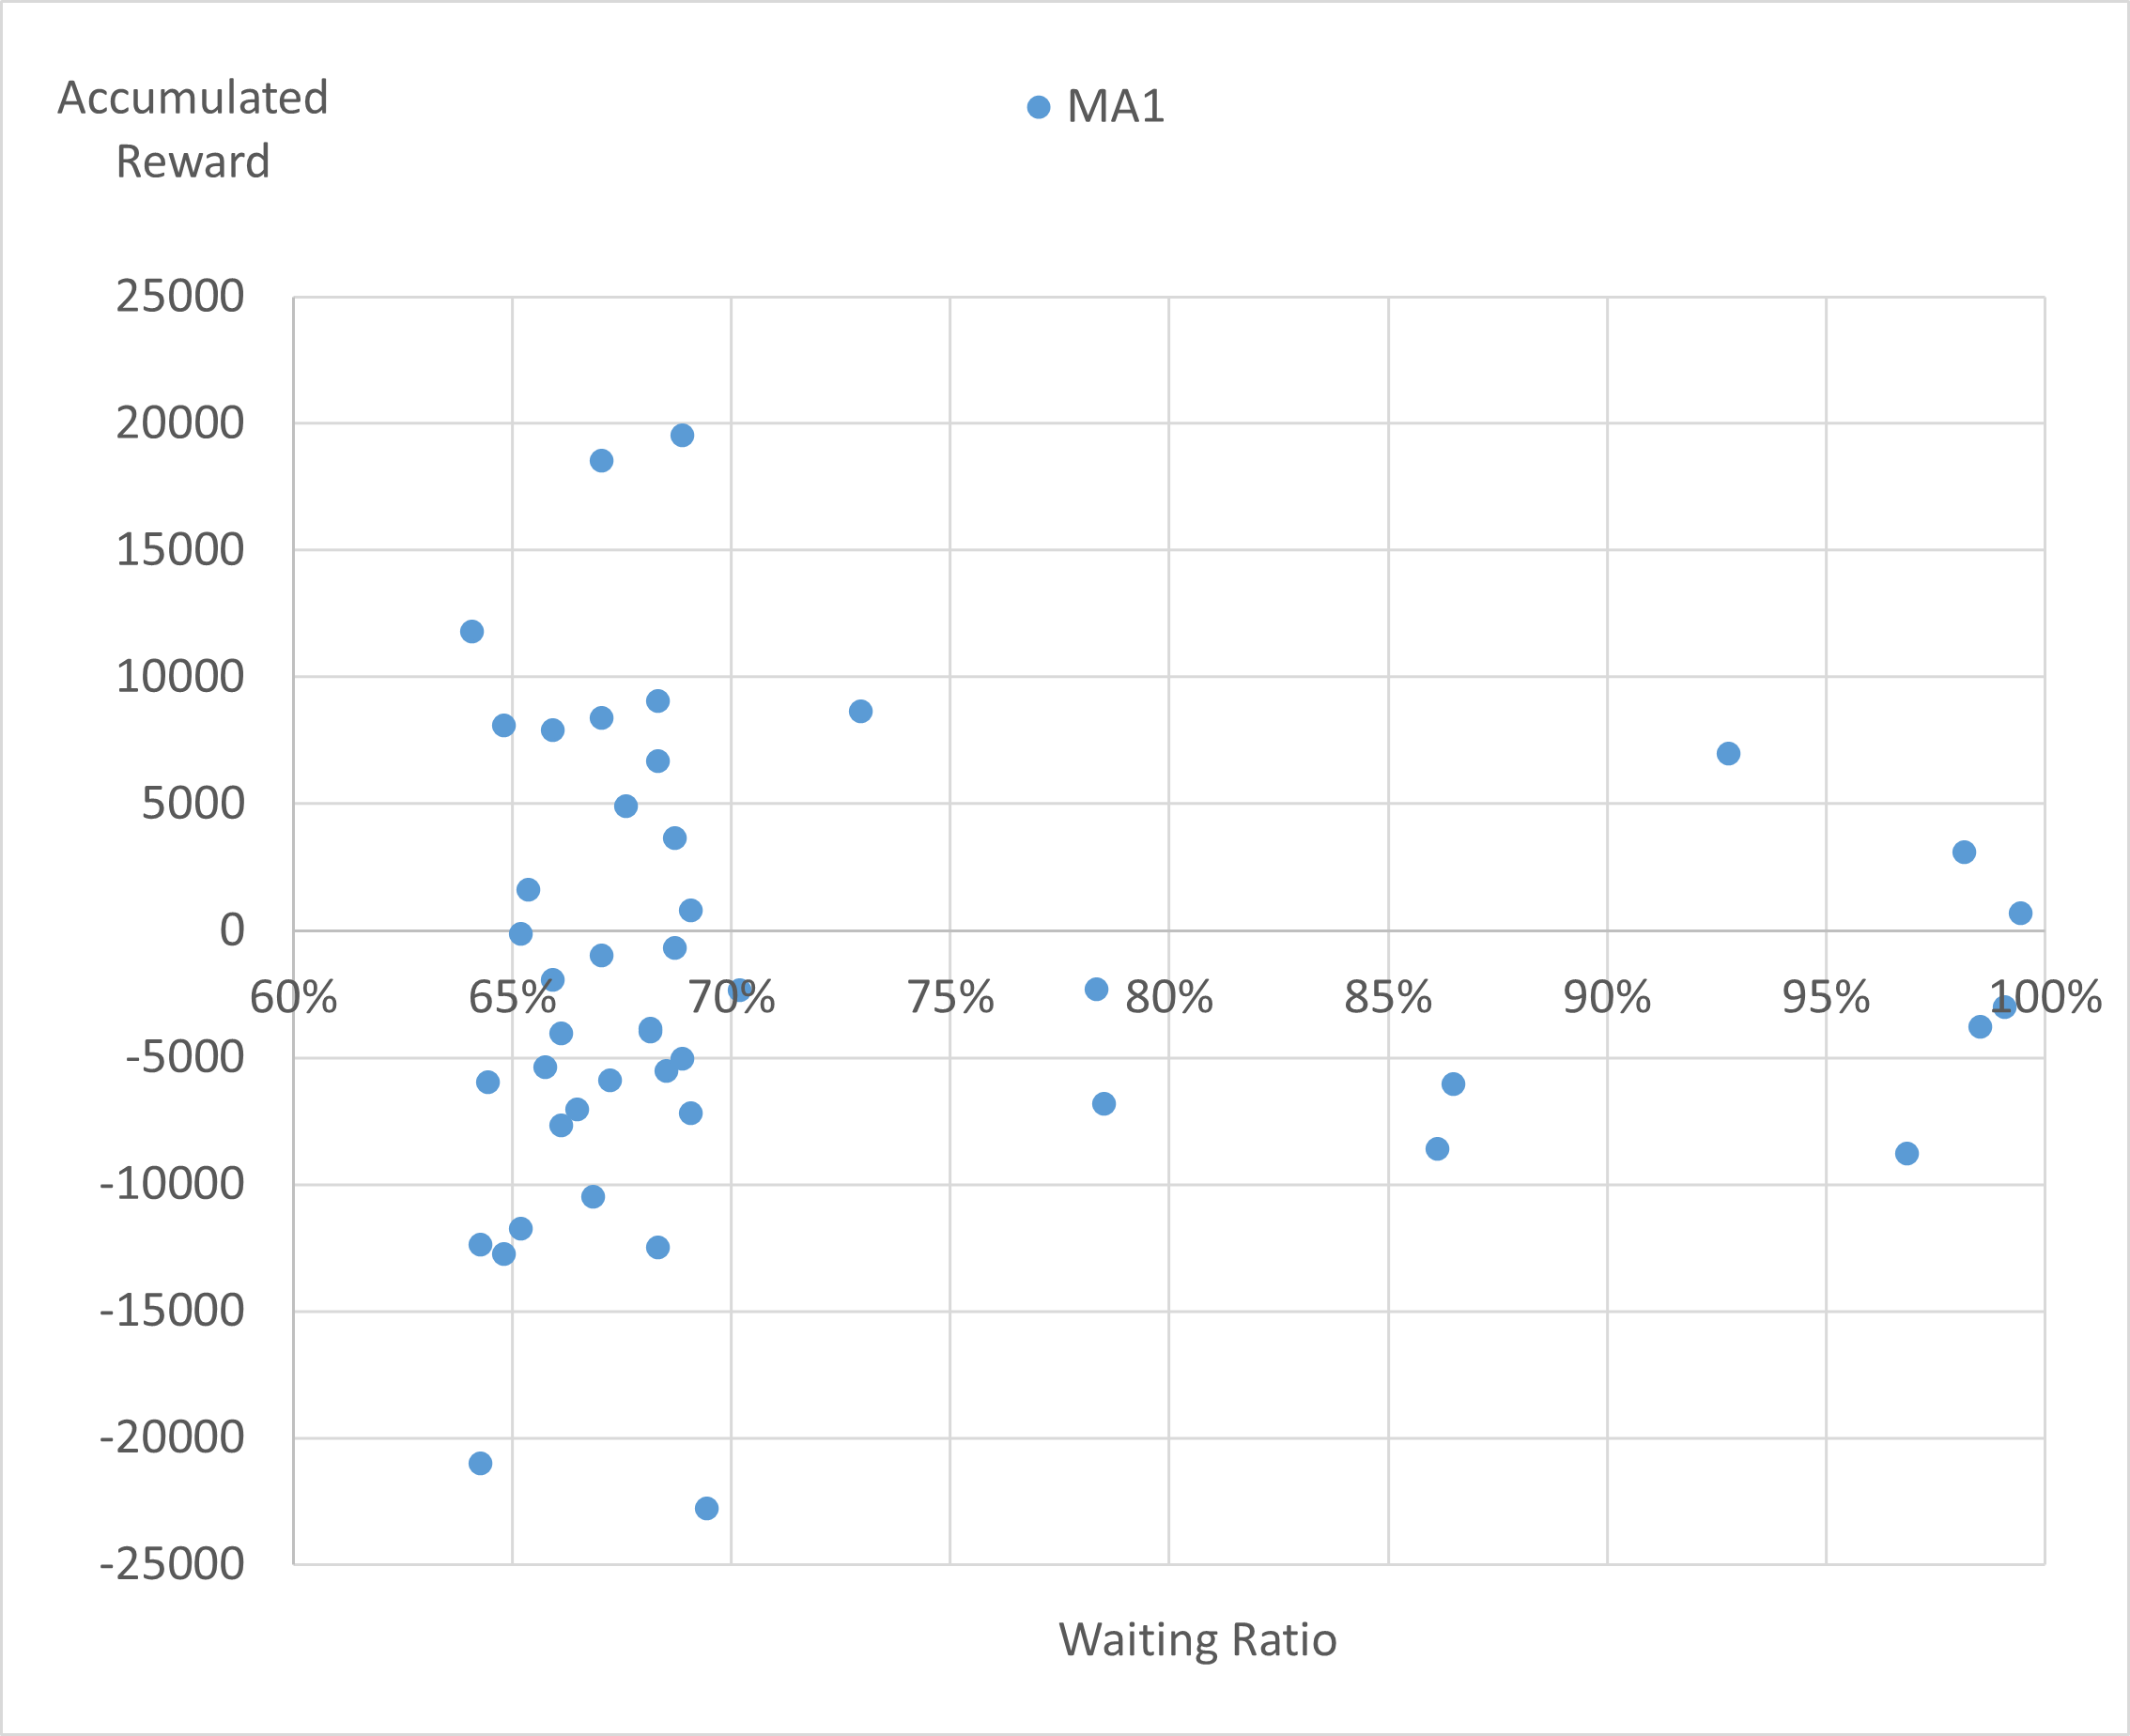
\includegraphics[scale=0.5]{./Figure/ma1waitingReward.png}
  \caption{Scatter plot between waiting ratio and accumulated reward in training of MA1}
  \label{fig:ma1waitingReward}
\end{figure}

\begin{figure}[htbp]
  \centering
  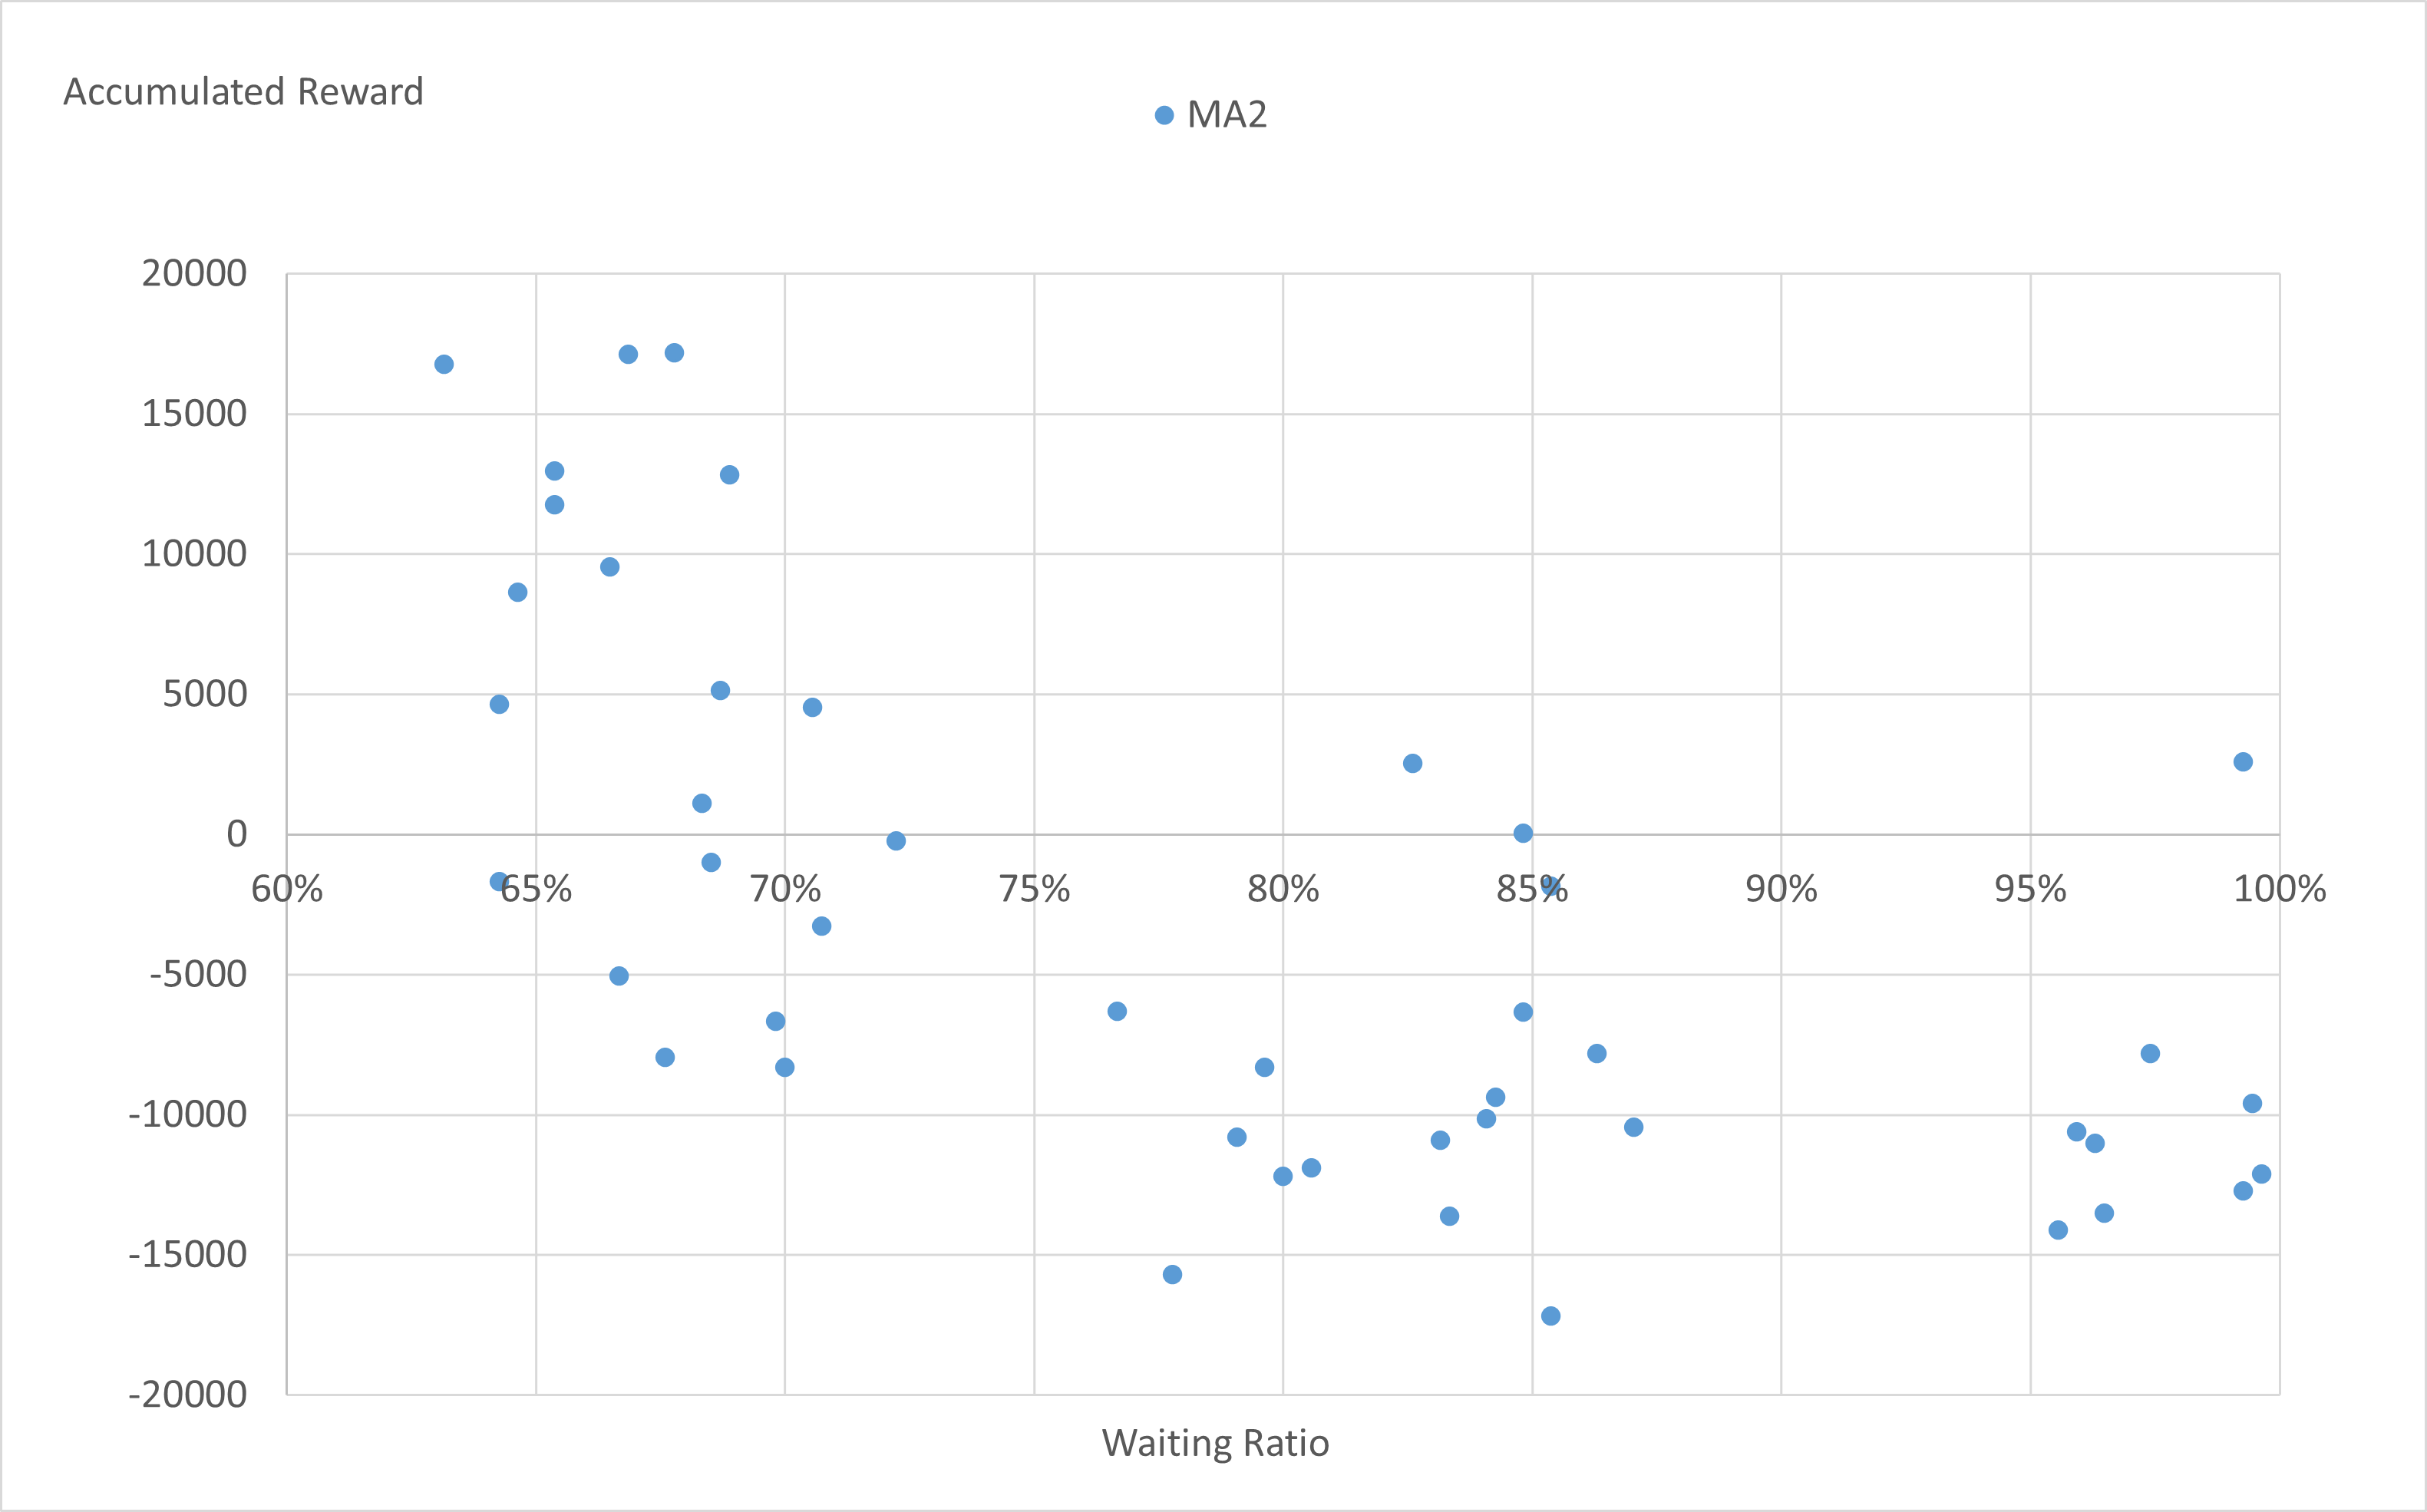
\includegraphics[scale=0.5]{./Figure/ma2waitingReward.png}
  \caption{Scatter plot between waiting ratio and accumulated reward in training of MA2}
  \label{fig:ma2waitingReward}
\end{figure}

\begin{figure}[htbp]
  \centering
  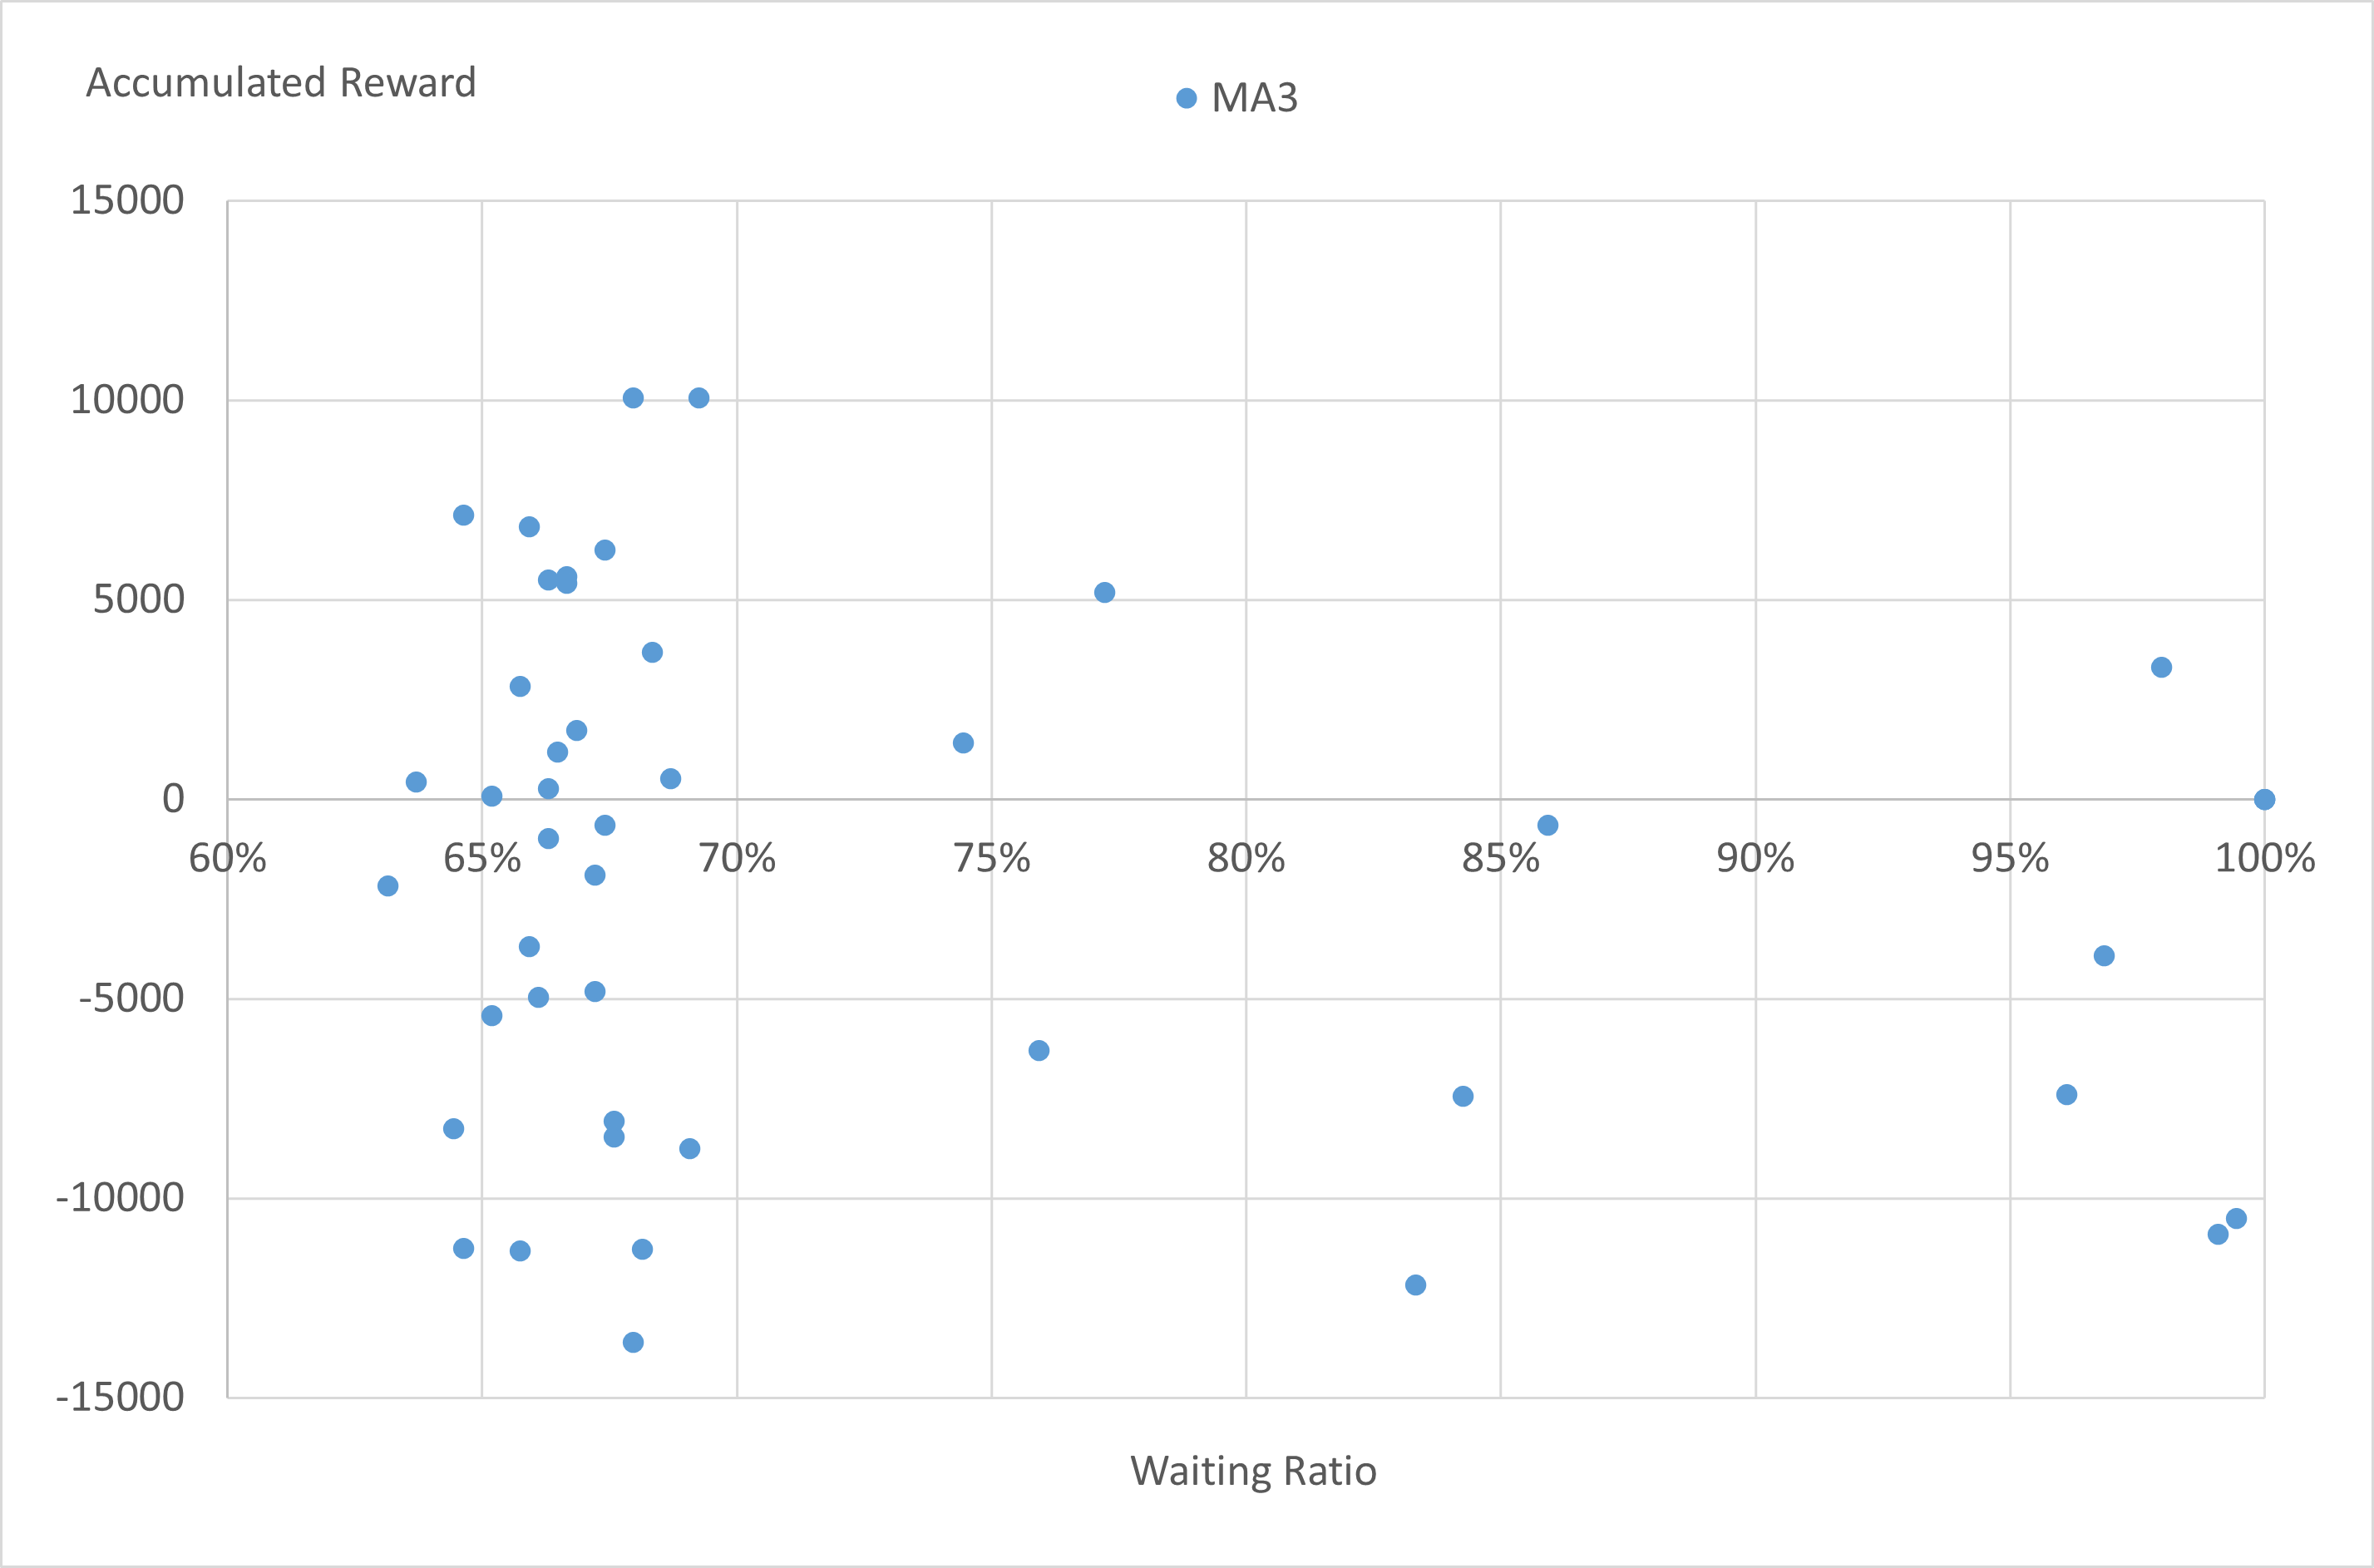
\includegraphics[scale=0.5]{./Figure/ma3waitingReward.png}
  \caption{Scatter plot between waiting ratio and accumulated reward in training of MA3}
  \label{fig:ma3waitingReward}
\end{figure}

\begin{figure}[htbp]
  \centering
  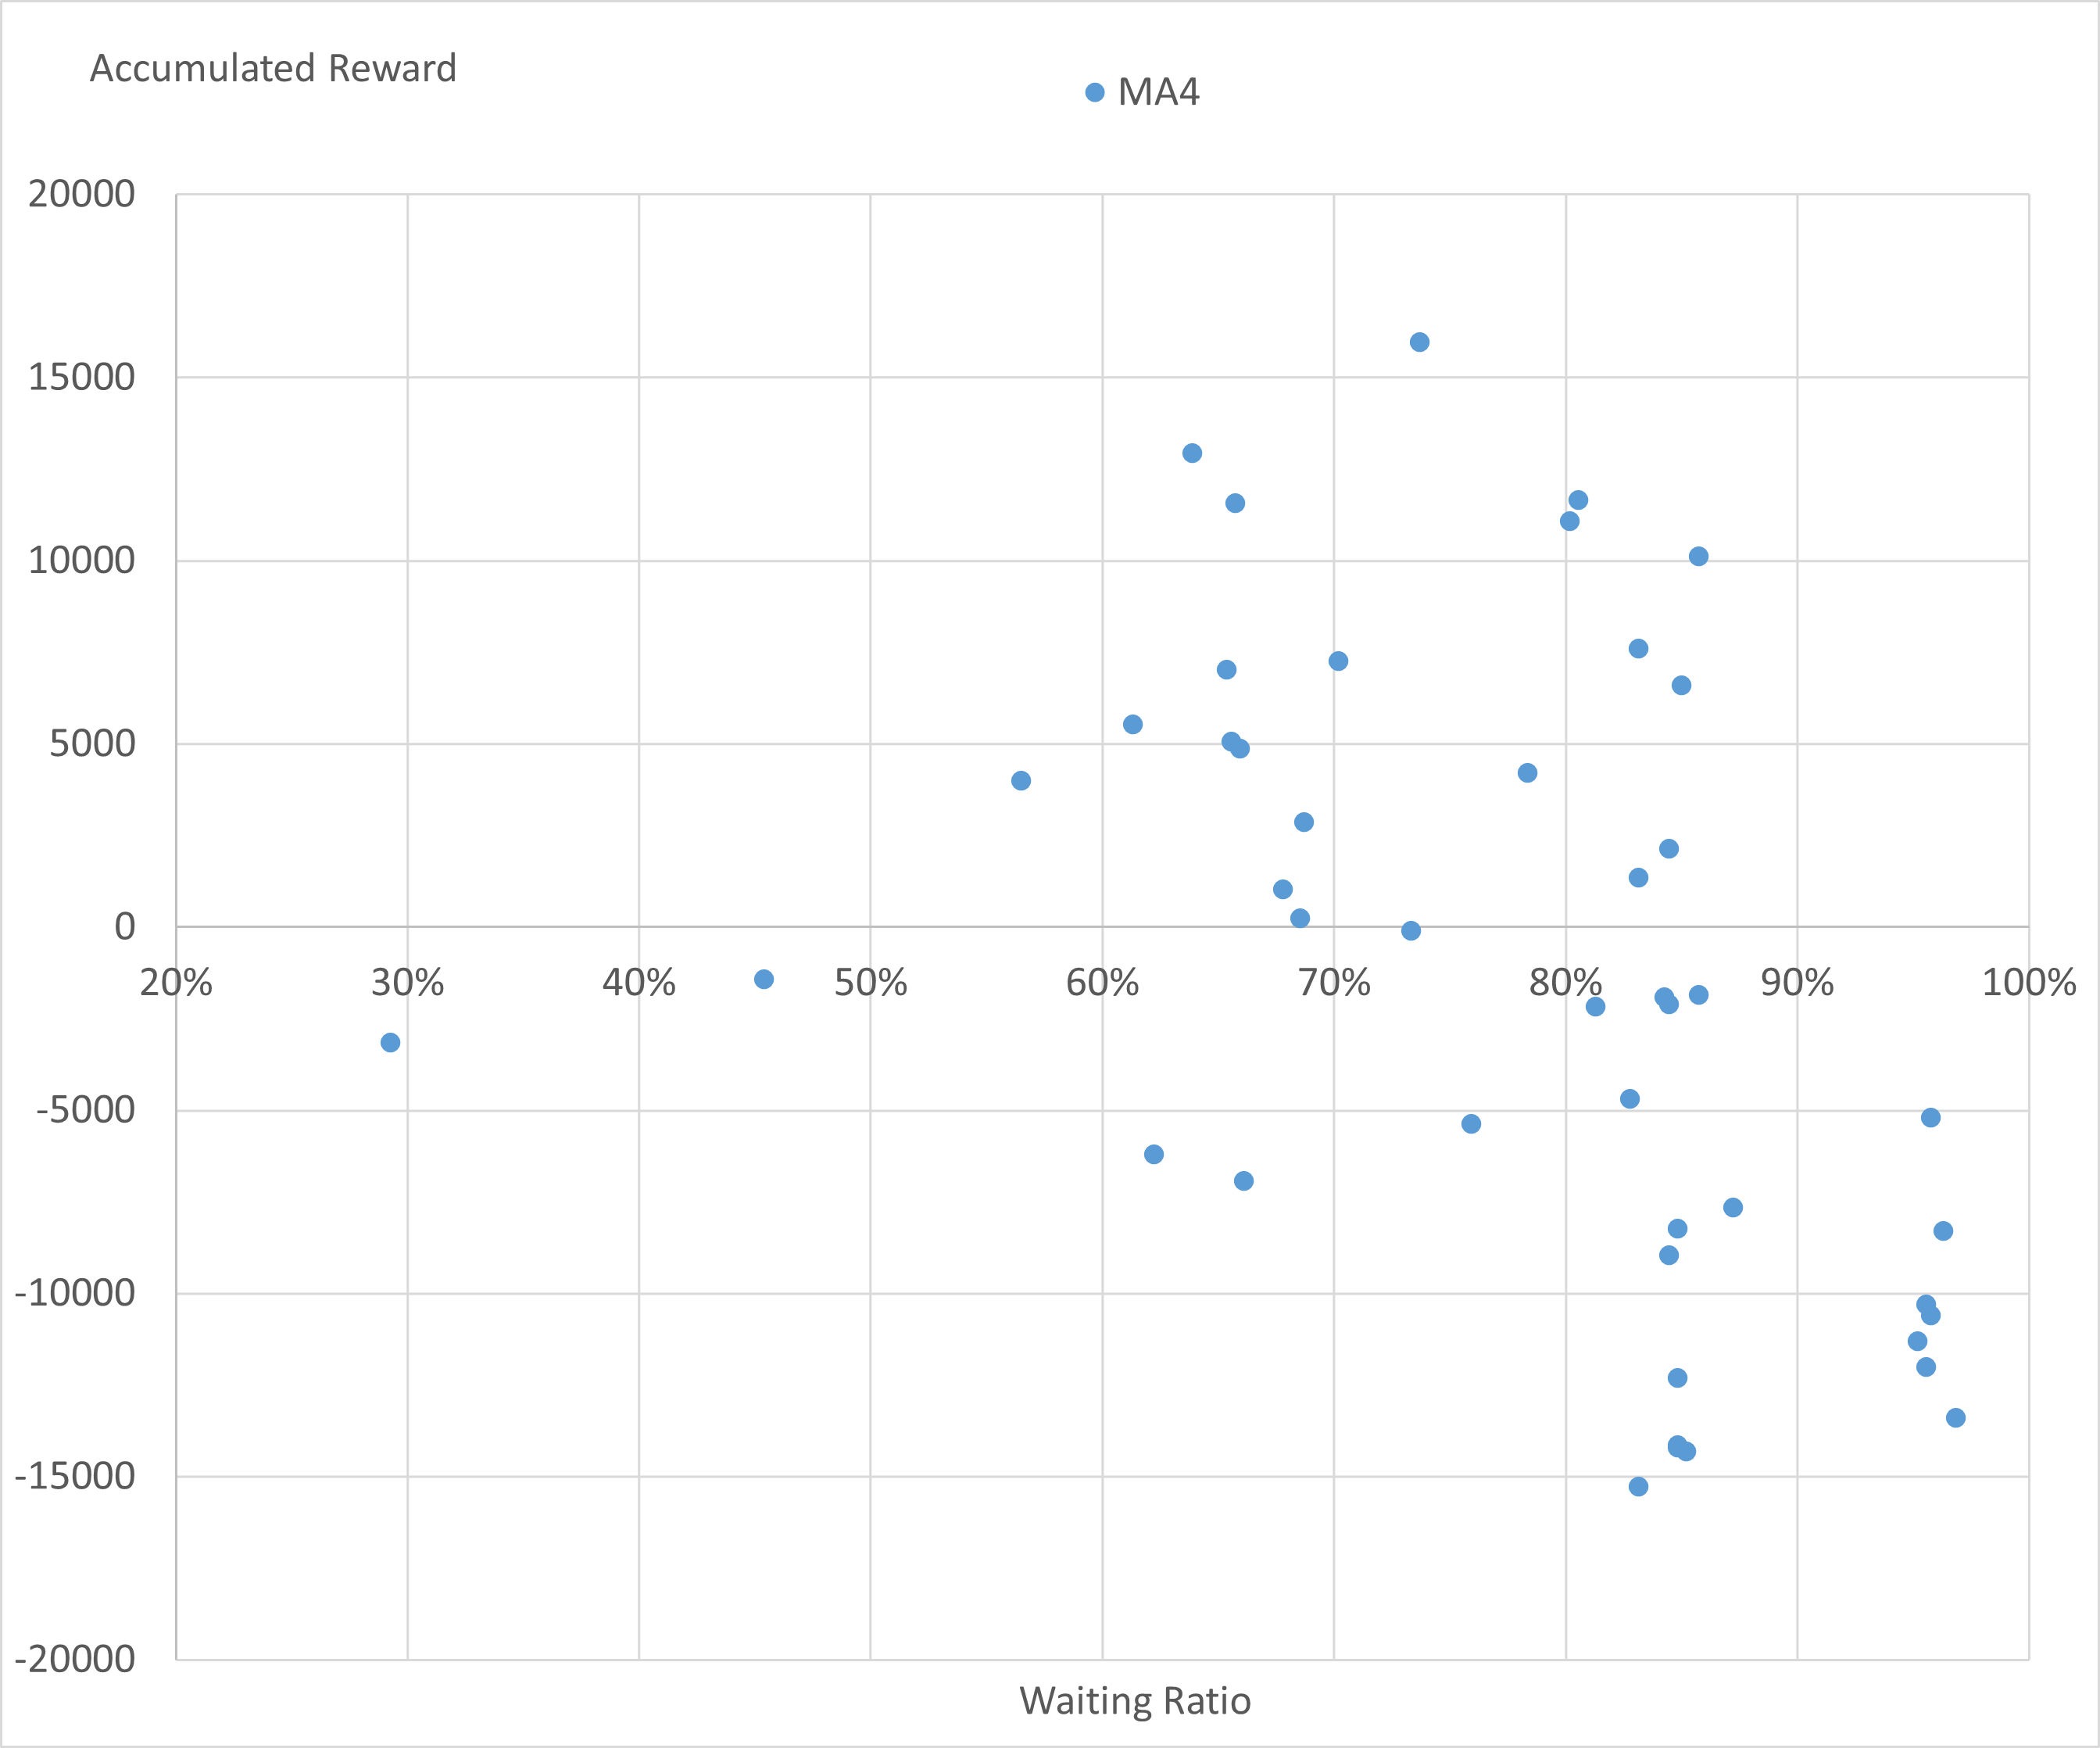
\includegraphics[scale=0.5]{./Figure/ma4waitingReward.png}
  \caption{Scatter plot between waiting ratio and accumulated reward in training of MA4}
  \label{fig:ma4waitingReward}
\end{figure}

\begin{figure}[htbp]
  \centering
  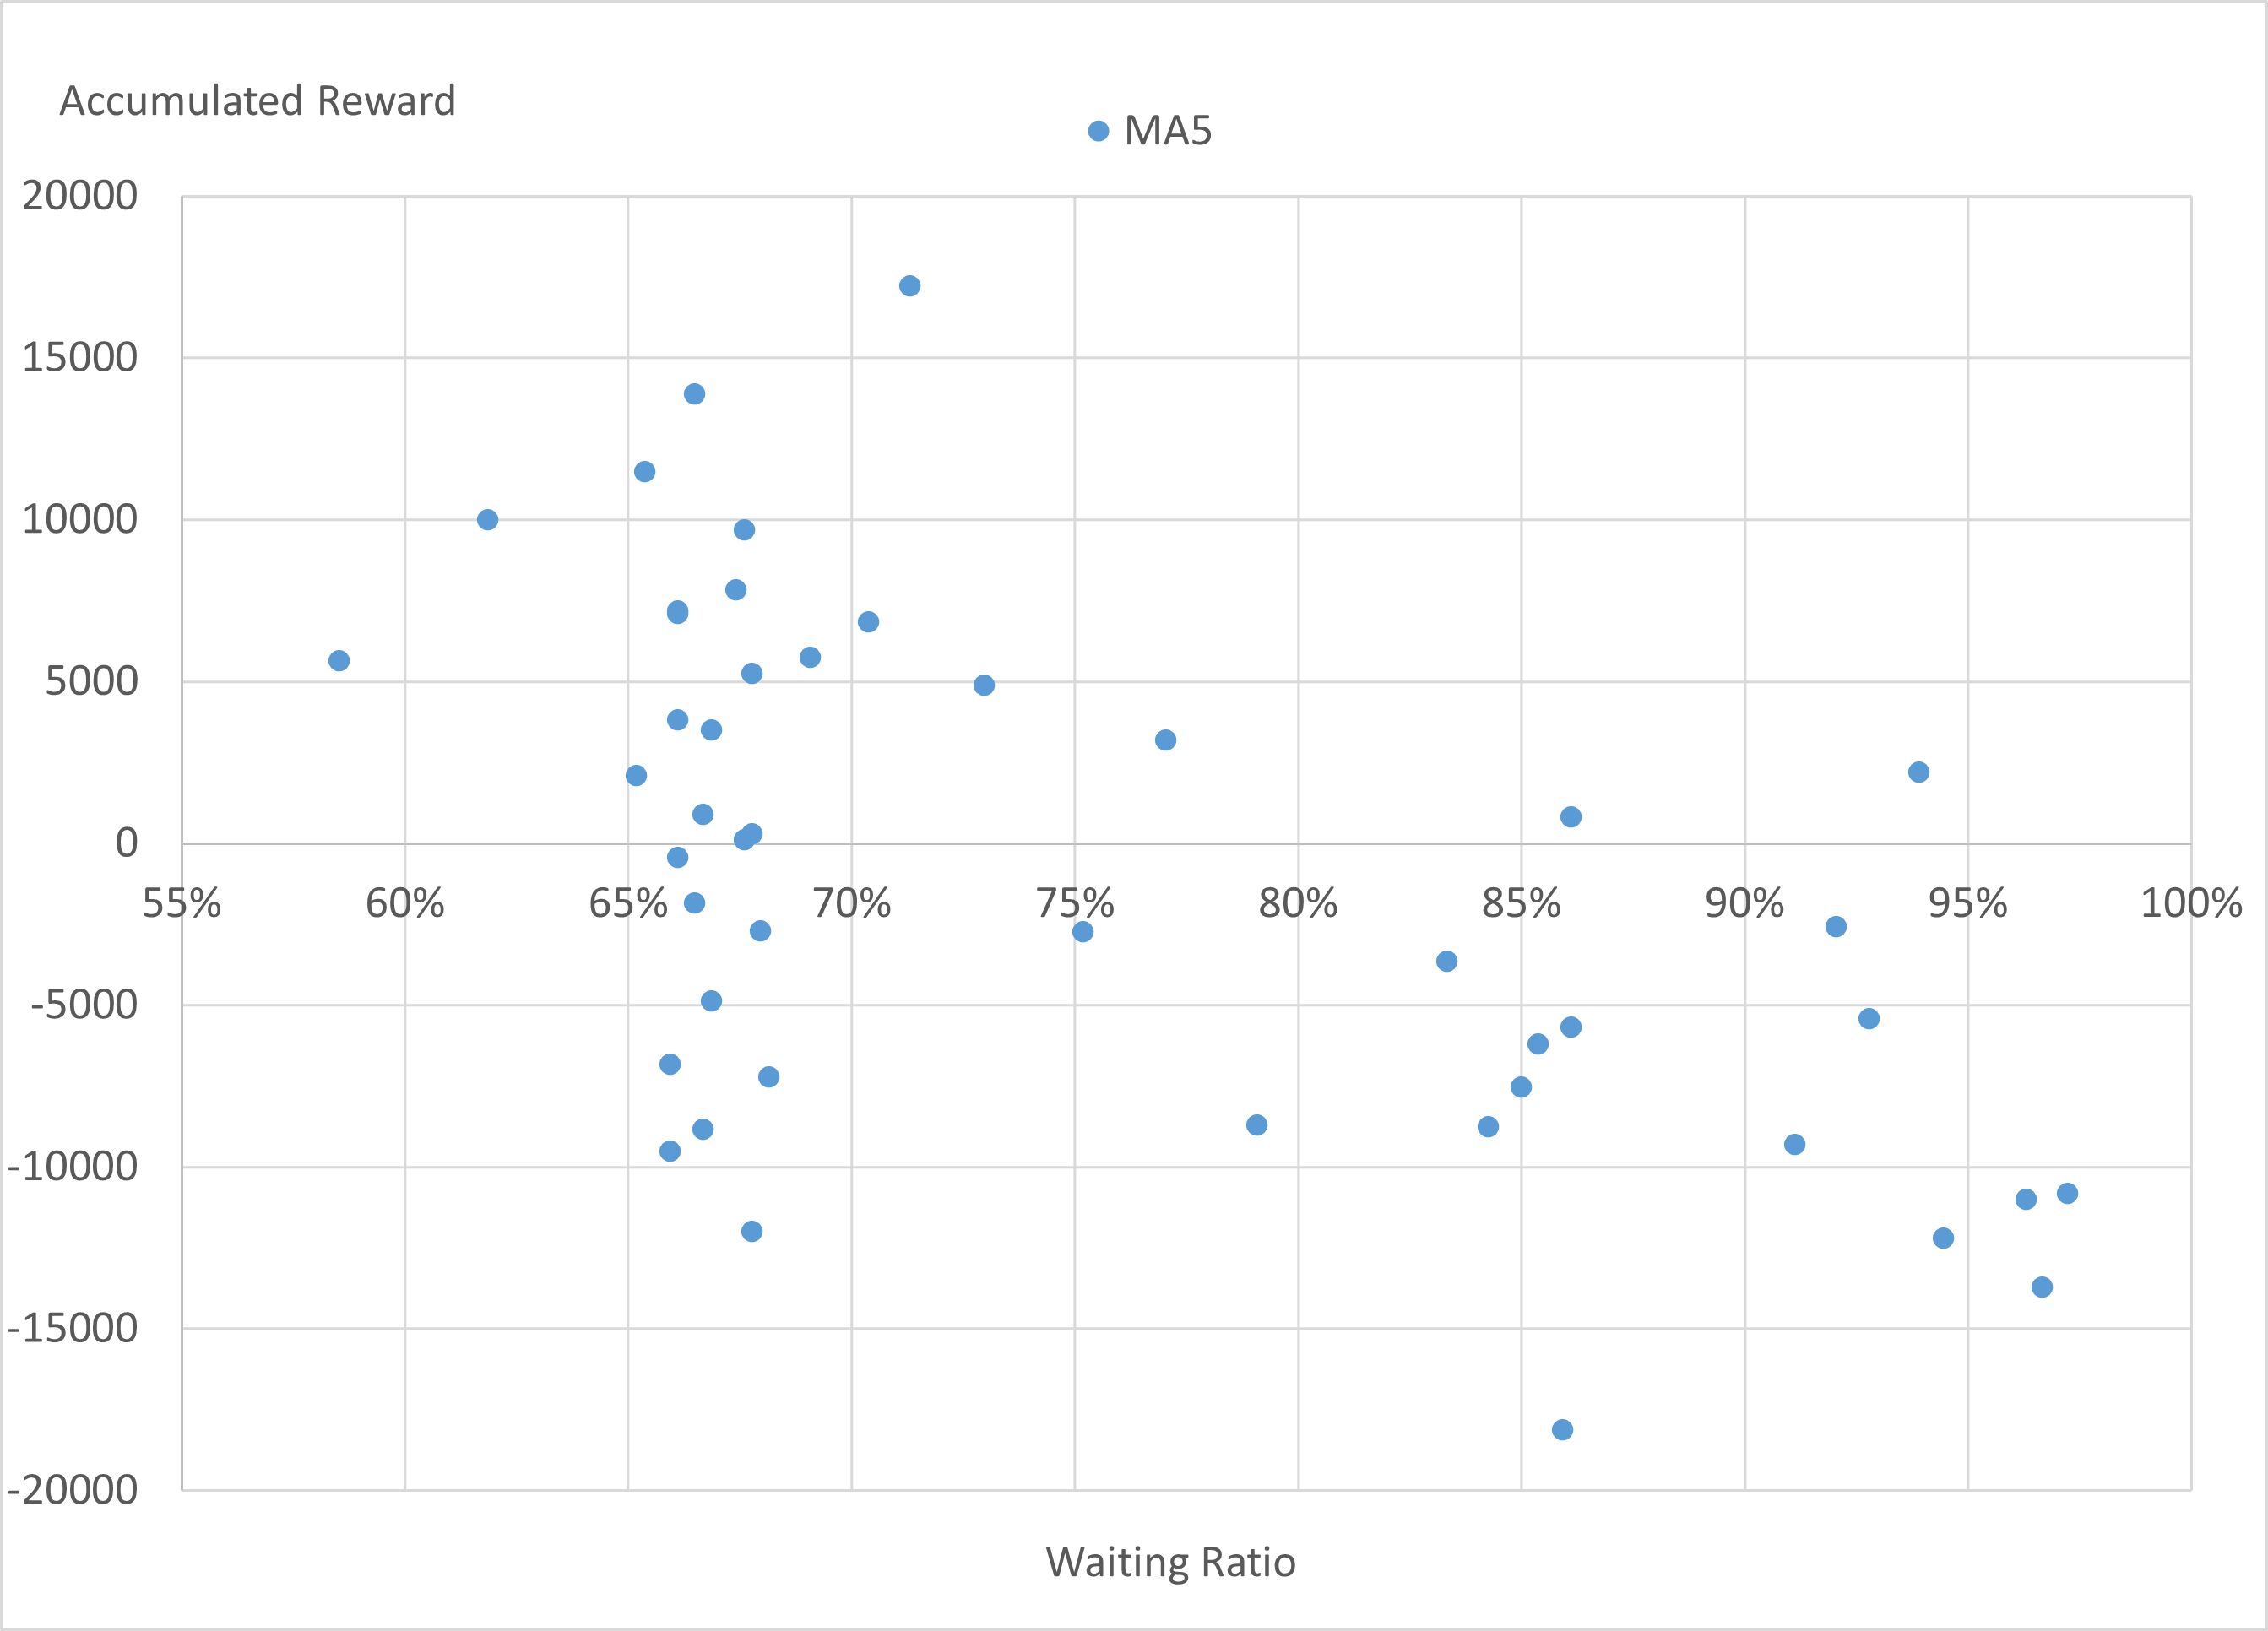
\includegraphics[scale=0.5]{./Figure/ma5waitingReward.png}
  \caption{Scatter plot between waiting ratio and accumulated reward in training of MA5}
  \label{fig:ma5waitingReward}
\end{figure}

Figure \ref{fig:waitingTest} and \ref{fig:waitingTestAvg} are consistent with the expectation of Section \ref{sec:evaluation}: the further the period of testing dataset is from the training period, the more the waiting ratio increases. The waiting can prevent losses when the agent cannot expect the future exchange rate.

In conclusion, RL itself is considered to be useful for avoiding losses in Forex trading.

\begin{figure}[htbp]
  \centering
  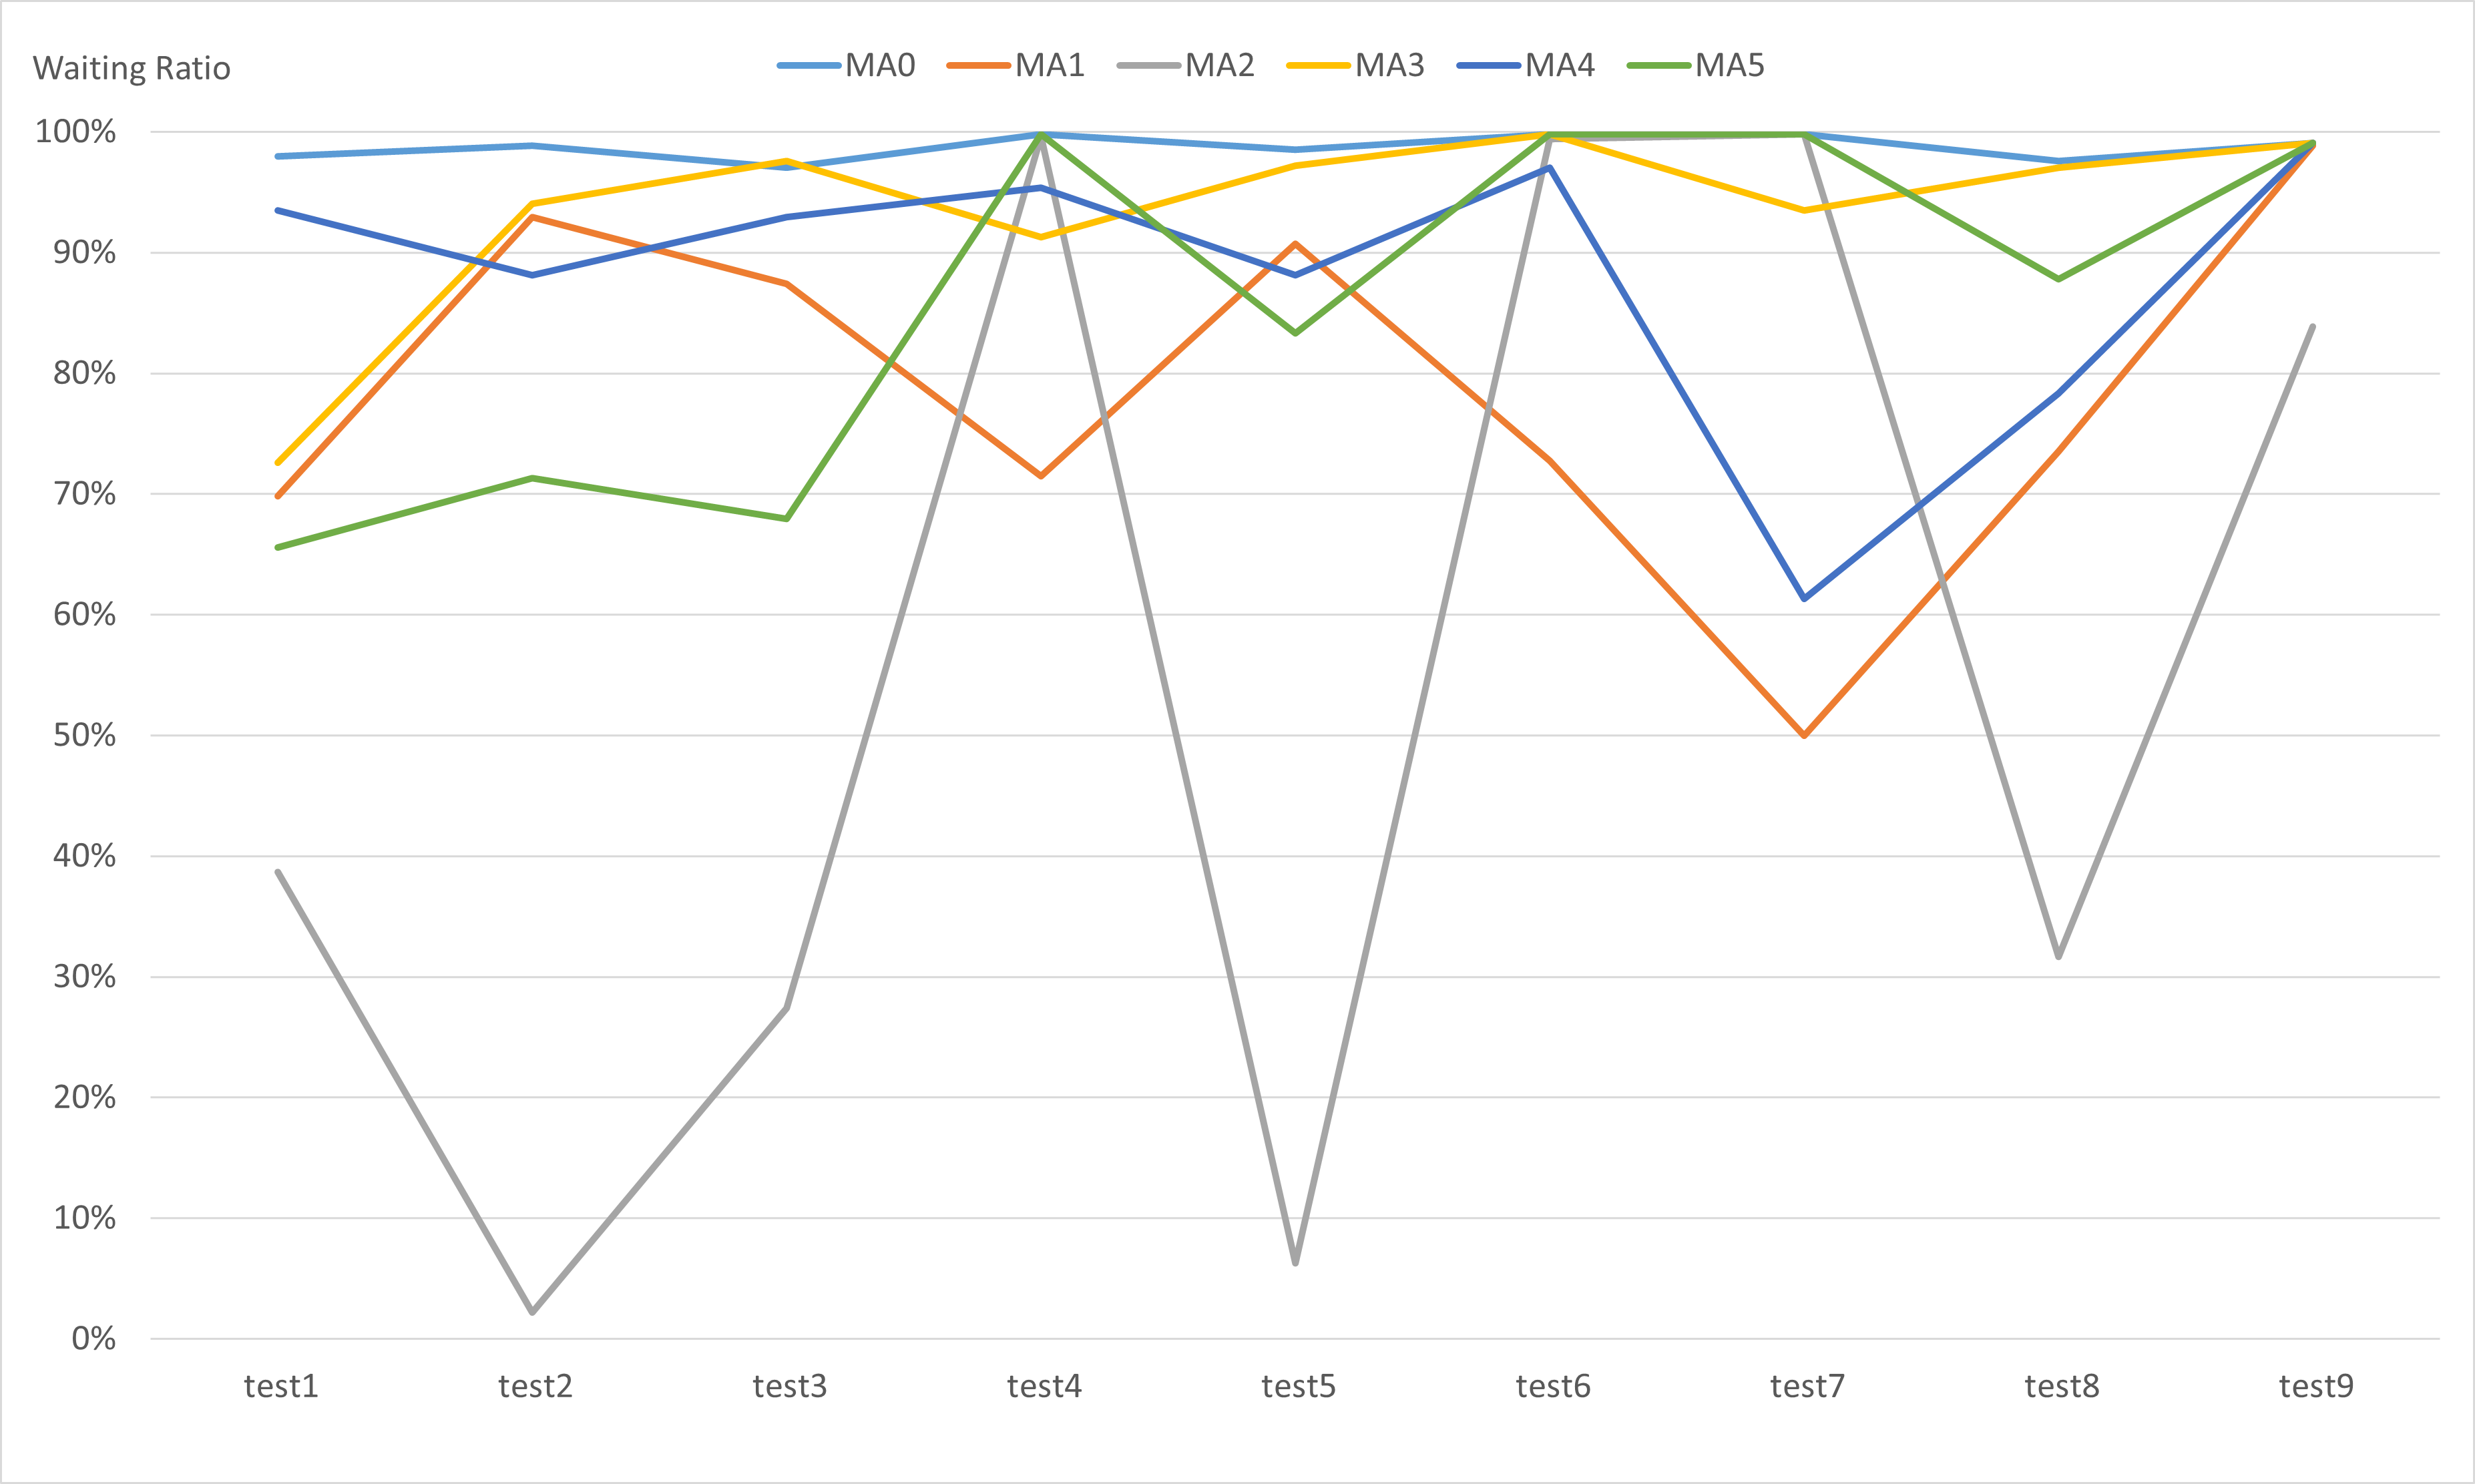
\includegraphics[scale=0.5]{./Figure/waitingTest.png}
  \caption{Waiting ratio in testing for the number of MA}
  \label{fig:waitingTest}
\end{figure}

\begin{figure}[htbp]
  \centering
  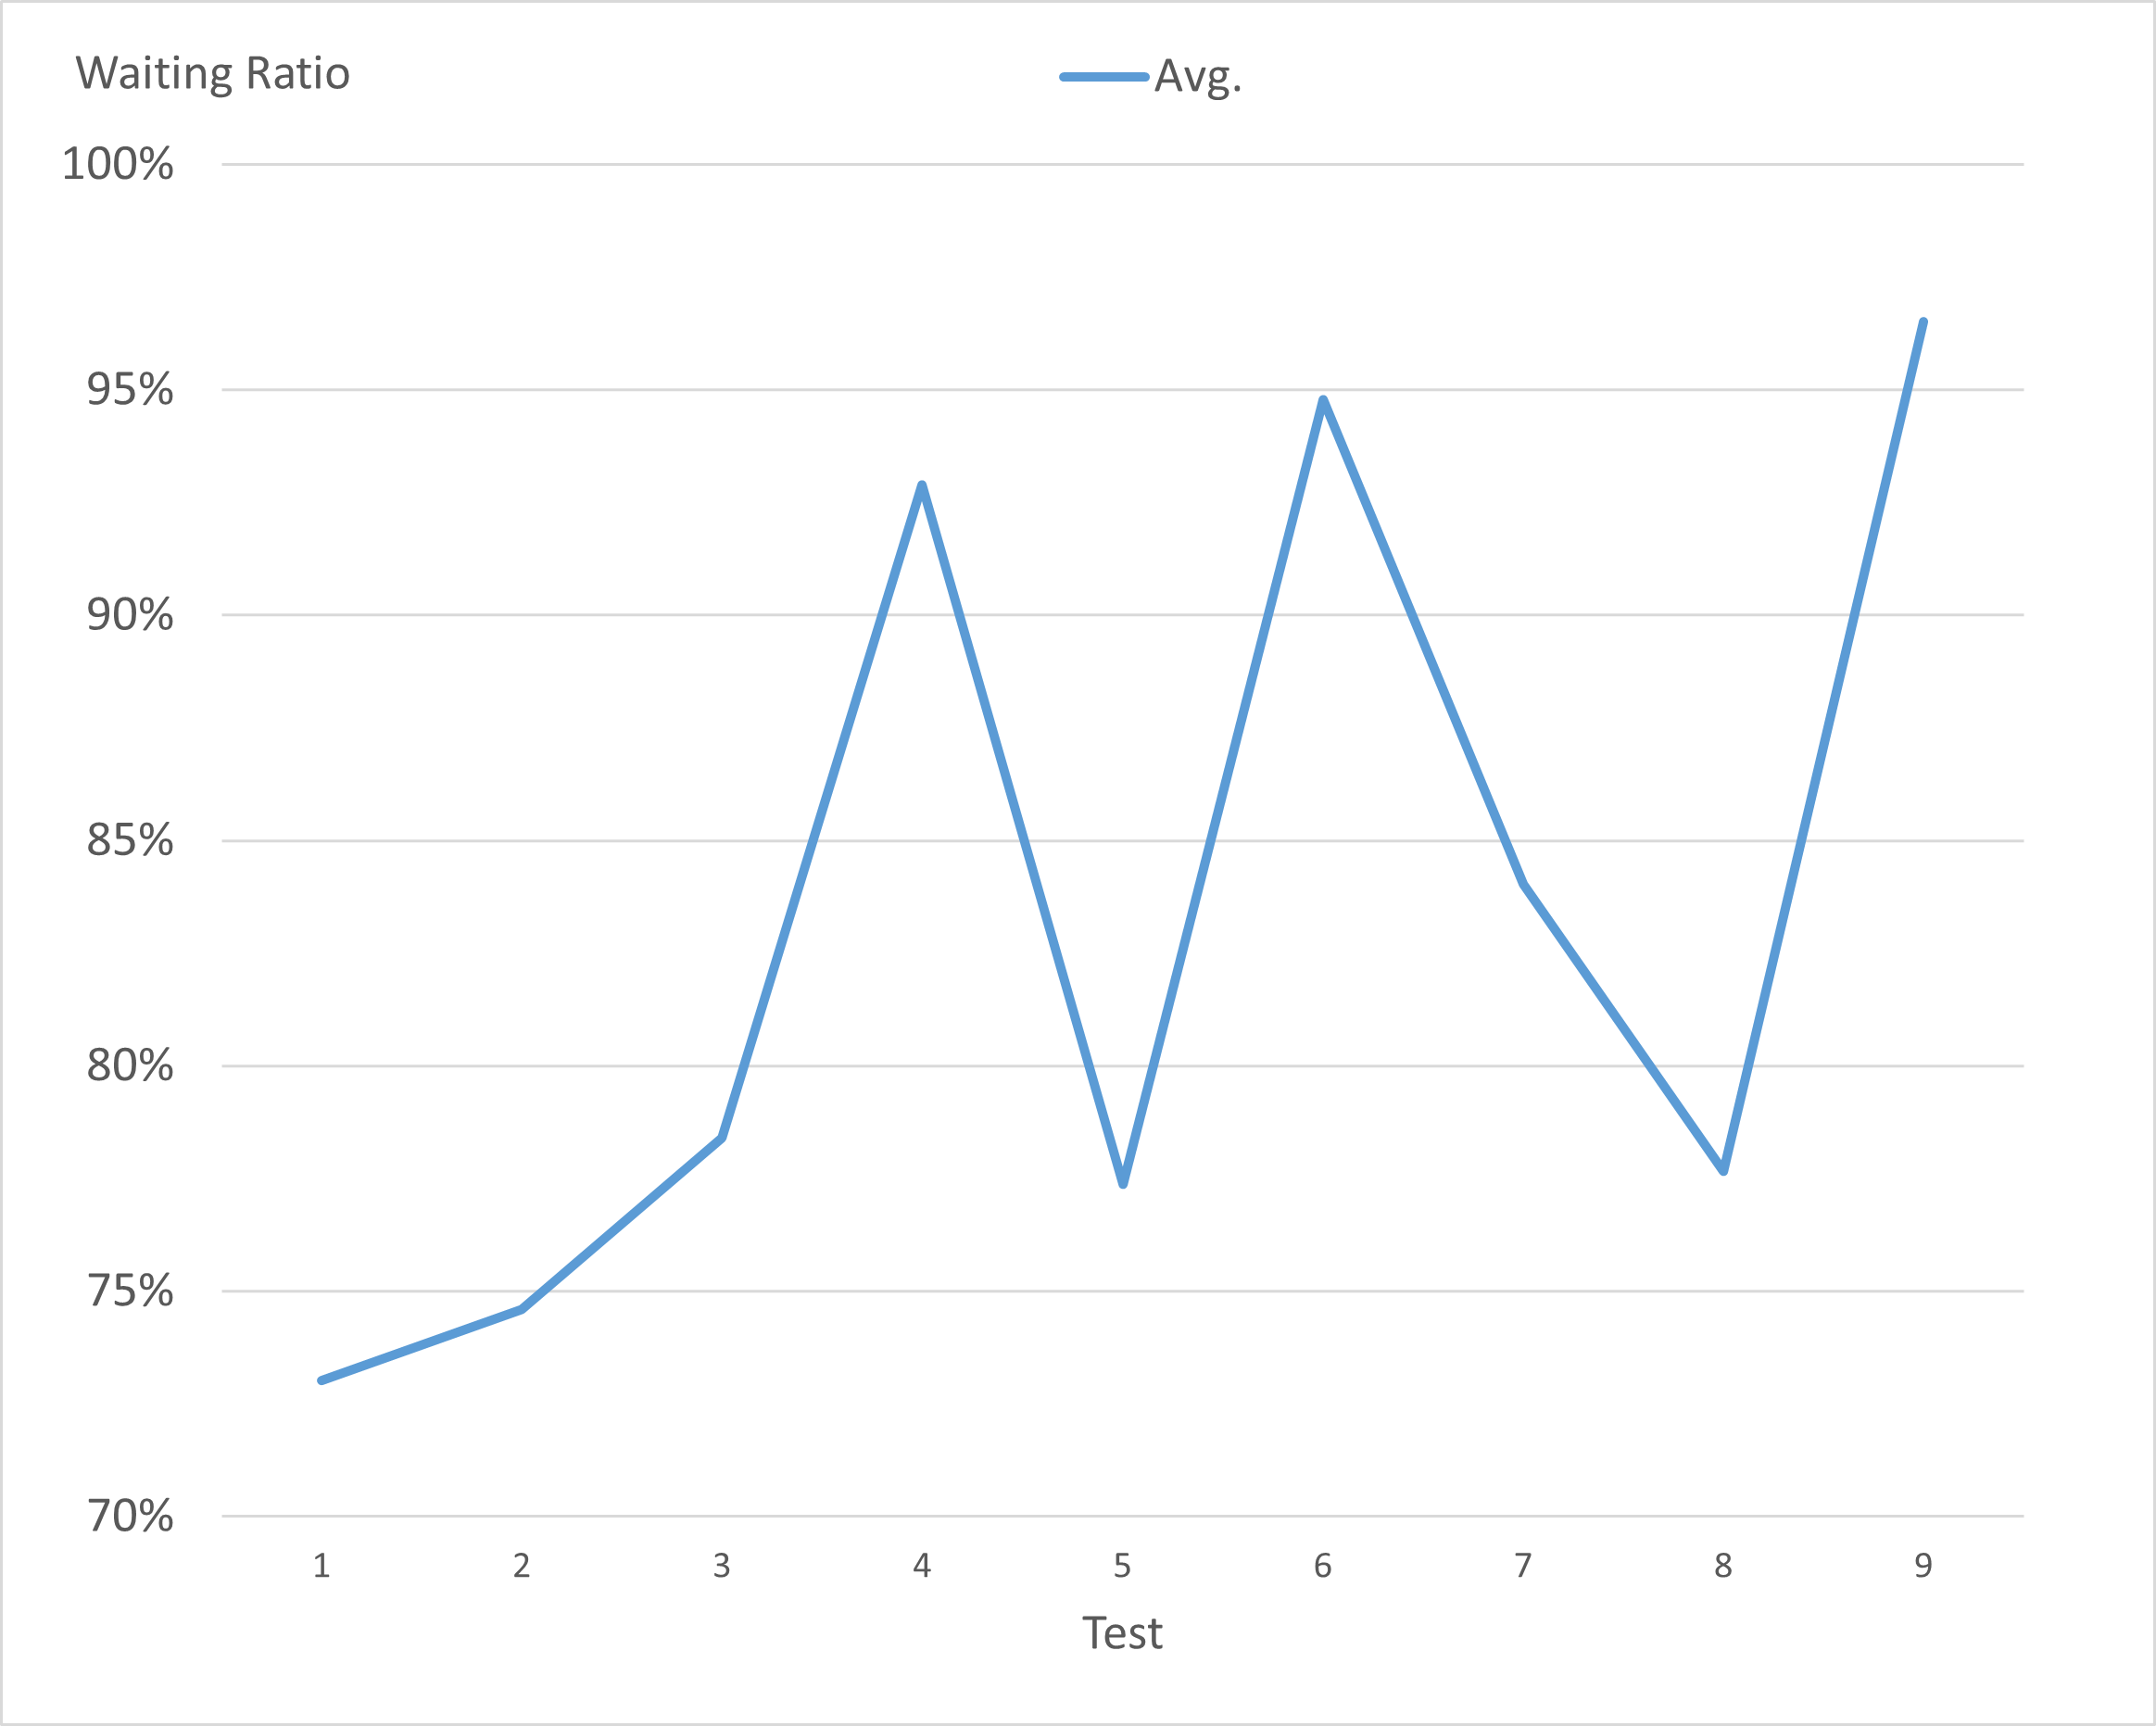
\includegraphics[scale=0.6]{./Figure/waitingTestAvg.png}
  \caption{Average of waiting ratio in testing}
  \label{fig:waitingTestAvg}
\end{figure}
